\documentclass{article}

%文章相关
\usepackage[UTF8, heading = false, scheme = plain]{ctex}    %解决中文字体,不改变排版
\usepackage{geometry}                                       %调整页边距等
\usepackage{indentfirst}                                    %首行缩进
\usepackage[dvipsnames,svgnames]{xcolor}                    %颜色包:\color{}
\usepackage{enumitem}                                       %控制item的前置符号
\usepackage{adjustbox}                                      %控制文字大小和添加底纹


%图片宏包
\usepackage{graphicx}                                       %插入图片:\includegraphics{myimage.png}
\usepackage{float}
\usepackage{caption}
\usepackage{subcaption}

%数学相关
\usepackage{amsmath,amsthm}                                 %amsmath包应该在前
\usepackage{extarrows}                                      %使用长等号A \xlongequal{\quad\quad}B
\usepackage{cases}                                          %\begin{numcases}可以为方程编号
\usepackage{amssymb}                                        %\checkmark 打勾

%实用的内容说明包
\usepackage{hyperref}                                       %超链接插入包:\href{url}{name}
\usepackage{multirow}                                       %插入表格用到的宏包:\begin{tabular}{|c|c|},&分列,\\分行,\hline插入横线(第二个参数是列数)
\usepackage{listings}                                       %插入代码等:\begin{lstlisting}[breaklines=true,backgroundcolor=\color{lightgray},title=]
\usepackage{verbatim}                                       %使用 comment 环境进行注释


%物理包
\usepackage{physics}
\usepackage{xparse}                                         %physics需求的包
\usepackage{mhchem}                                         %输入原子核的表式\ce{^238_92U}

% \eval{}        根据括号内容的大小在右边添加合适的竖线A|          |         \dv[n]{f}{x}          n阶微分算符 derivative
% \abs{}         添加绝对值|A|                                |         \pdv[n]{f}{x}         n阶偏微分算符 partialderivative
% \norm{}        模||A||                                     |          \bra \ket \braket    左、右、内积
% \comm{}{}      对易子[A,B]                                  |          \op{}{}              外积(密度算符) outerproduct
% \anticomm{}{}  反对易子{A,B}                                |          \ev{<力学量>}{<态>}    期望 expectationvalue
% \vb{}          向量加粗字体                                  |          \mel{}{}{}           矩阵元 matrixelement
% \va{}          向量                                        |          \mqty                 生成矩阵,可跟{} () [] || &分列 \\分行 第一个表示外面无框
% \vu{}          单位向量                                     |         \qty                  合适大小的{}、()等,例如 \qty(x)
% \vdot          点乘                                        |
% \cross         叉乘                                        |
% \grad          梯度 gradient                               |
% \div           散度 divergenc                              |
% \curl          旋度                                        |
% \laplacian     拉普拉斯算符                                 |

%文本底纹实现
\usepackage{lipsum}                                         %该宏包是通过 \lipsum 命令生成一段本文,正式使用时不需要引用该宏包
\usepackage[strict]{changepage}                             %提供一个 adjustwidth 环境
\usepackage{framed}                                         %实现方框效果
%\usepackage{newtxtext}                                     %在macos会报错的一个包注释掉不影响使用
\usepackage{tcolorbox}                                      %文本底纹包,放在xcolor包后
                               
% environment derived from framed.sty: see leftbar environment definition
\definecolor{formalshade}{rgb}{0.95,0.95,1}% 文本框颜色
% ------------------******-------------------
% 注意行末需要把空格注释掉,不然画出来的方框会有空白竖线
\newenvironment{formal}{%
\def\FrameCommand{%
\hspace{-1em}%                                              %框的整体缩进
{\color{Green}\vrule width 0.3em}%                          %竖线颜色以及宽度
\colorbox{greenshade}%                                      %底纹颜色
}%
\MakeFramed{\advance\hsize-\width\FrameRestore}%
\noindent\hspace{-2em}%                                     %禁止第一段文本缩进
\begin{adjustwidth}{}{2em}%                                 %控制右边距        
\vspace{1.5em}%                                             %控制上边距
}
{%
\vspace{1.5em}\end{adjustwidth}\endMakeFramed%              %控制底边距
}%

\definecolor{greenshade}{rgb}{0.90,0.99,0.91}               %绿色文本框,竖线颜色设为 Green
\definecolor{redshade}{rgb}{1.00,0.90,0.90}                 %红色文本框,竖线颜色设为 LightCoral
\definecolor{brownshade}{rgb}{0.99,0.97,0.93}               %莫兰迪棕色,竖线颜色设为 BurlyWood


%使用Mathematica进行计算
%\usepackage{latexalpha2}
%/usr/local/texlive/texmf-local/tex/latex/local/latexalpha2
%直接使用wolfram代码
% \wolfram[<format>]{<code>}    \wolframgraphics[<format>]{<code>}{<filename>} 
%具体使用方法查看 latexalpha2.pdf


%预设
\geometry{a4paper,left=5em,right=5em,bottom=5em,top=5em}    %设置为a4paper最好,点击pacakge geometry 查看文档
\setlength{\parindent}{2em}                                 %2em(注意不支持rem)代表每一段的首行缩进两个字符,某一行不缩进时使用 \noindent

\hypersetup{hidelinks,colorlinks=true,
linkcolor=black,urlcolor=blue}                              %对hyperref 包进行预设

\newenvironment{slt}{\proof[\indent \bf 解 ]}{
\renewcommand{\qedsymbol}{}\endproof}                       %提供解环境
\newtheorem{thm}{定理}[section]                              %定义一个新的环境 thm, 命名为定理,以 节 开始编号
\newtheorem*{thm*}{定理}                                     %定义一个新的环境 thm, 命名为定理,无编号
\newtheorem{lemma}{引理}[section]                            %定义新环境 lemma,命名为引理,以 节 开始编号
\newtheorem*{lemma*}{引理}                                   %定义新环境 lemma,命名为引理,无编号
\newtheorem{corollary}{推论}                                 %定义新环境 corollary,命名为推理,有编号
\newtheorem*{corollary*}{推论}                               %定义新环境 corollary*,命名为推理,无编号
\renewcommand{\proofname}{ \qquad \bf 证明}                  %更改proof为中文证明,proof环境默认存在

%一些def
\def\thmindent{\setlength{\parindent}{5em}}                  %\thmindent
\def\pfindent{\setlength{\parindent}{5.5em}}                 %\pfindent
\def\clindent{\setlength{\parindent}{4em}}                   %clindent
\def\sdr{Schr\"{o}dinger}                                    %薛定谔名字
\def\intff{\int_{-\infty}^{+\infty}}                         %积分为(-\infty,+\infty)的积分
\def\ra{\rightarrow}                                         %右键头\ra
\def\lra{\Longrightarrow}                                    %长(双)右键头\lra
\def\lla{\Longleftarrow}                                     %长(双)左键头\lla
\def\llra{\Longleftrightarrow}                               %等价箭头\llra
\def\xlra{\xlongrightarrow{\quad\quad}}                      %超长右箭头
\def\xlla{\xlongleftarrow{\quad\quad}}                       %超长左箭头
\def\xlla{\xlongleftrightarrow{\quad\quad}}                  %超长等价箭头

\def\psii#1{\psi_{#1}}                                       %常用的\psi下标
\def\psiii#1#2{\psi_{#1} (#2)}                               %常用的\psi下标和括号
\def\psiiii#1#2#3{\psi_{#1}^{#2} (#3)}                       %常用的\psi下标、上标和括号
\def\pe#1#2{E_{#1}^{(#2)}}                                   %能量修正{下标}{上标}
\def\pp#1#2{\psi_{#1}^{(#2)}}                                %波函数修正
\def\ua{a_{+}}                                               %升算符
\def\da{a_{-}}                                               %降算符

\def\nuc#1#2#3{\ce{^{#1}_{#2}{#3}}}                          %原子核的表示形式


%其他备注
\begin{comment}
        求和指标上下方添加        \sum\limits_{}^{}
        恒等于                  \equiv
        远大于                  \gg
        远小于                  \ll
        花括号                  \left\{ \right\}   (建议使用\qty)
        弧度                    37^{\circ}


\end{comment}


%作业包(需要的时候再解除注释)
%\usepackage{iidef}
%建议使用自己的slt解环境
\begin{comment}

    package iidef:
        指定学校名      \thecourseinstitute{}      
        指定课程名      \thecoursename{} 
	    指定学期        \theterm{}
        作业名         \hwname{}
        生成作业标题    \courseheader           放在document环境内 不需要再maketile
        名字           \name                   放在document环境内
        自动编号环境    \begin{enumerate}       [label = (\alph*{})] [label = \arabic*{}.]
        题号           \item                   自动编号,\item[]则不带符号
        证明           \begin{proof}           证明环境由amsthm包提供
        求解           \begin{solution}       
        方程           \begin{equation}        
        方程编号        \labe{eq:[number]}      为方程设置编号  
        引用方程        \eqref{eq:[number]}     引用方程
        行内方程        $...$
        
        多行公式        \begin{align} \begin{align*}则不会编号  
                            ... & = ... \\ 
                                & = ...
                       \begin{array}{lcl}      
                            ... & = & ... \\ 
                            ... & = & ...
        
        方程组          $$
                        \begin{cases}
                       ... & \mbox{if} x \mbox{is even} \\ 带假设
                       $$
                       
                       带编号
                       \begin{numcases}{}
                            \label{1}   \\
                            \label{2}   
                       \end{numcases}
        
        文字大小和底纹
                       \vspace{-1em}
                       \begin{adjustbox}{minipage=0.91\linewidth, bgcolor=gray!20, padding=1em}
                       \small % 将字号变小为 small
                        text
                       \end{adjustbox}
                       \vspace{-1em}

        居中            不要使用$$...$$,会对齐失效 使用$...$即可
                        \begin{center}
            
                        \end{center}

        左对齐           
                        \begin{flushleft}
            
                        \end{flushleft}

        双水平图         \begin{minipage}{0.45\textwidth}
                        \includegraphics[width=\textwidth,keepaspectratio]{./pictures/.png}
                        \end{minipage}
                        \hfill
                        \begin{minipage}{0.45\textwidth}
                            \begin{enumerate}[label = (\arabic*)]
                                \item 
                                \item 
                                \item 
                            \end{enumerate}
                        \end{minipage}

    
\end{comment}




\begin{comment}
    重复语句
    \subsubsection{}
    \includegraphics[width=50em,keepaspectratio]{}

    \begin{itemize}
        \item 错选:\quad
        \item 正解:\quad
        \item 总结:\quad
        \item 扩展:\quad
    \end{itemize}

\end{comment}


\title{高中物理错题集}
\author{马祥芸}

\begin{document}
    \maketitle
    \tableofcontents
    \newpage

    \section{高一}  

    \subsection{2022-2023年度(下)重庆八中高一期末}

    \subsubsection{I-7}
    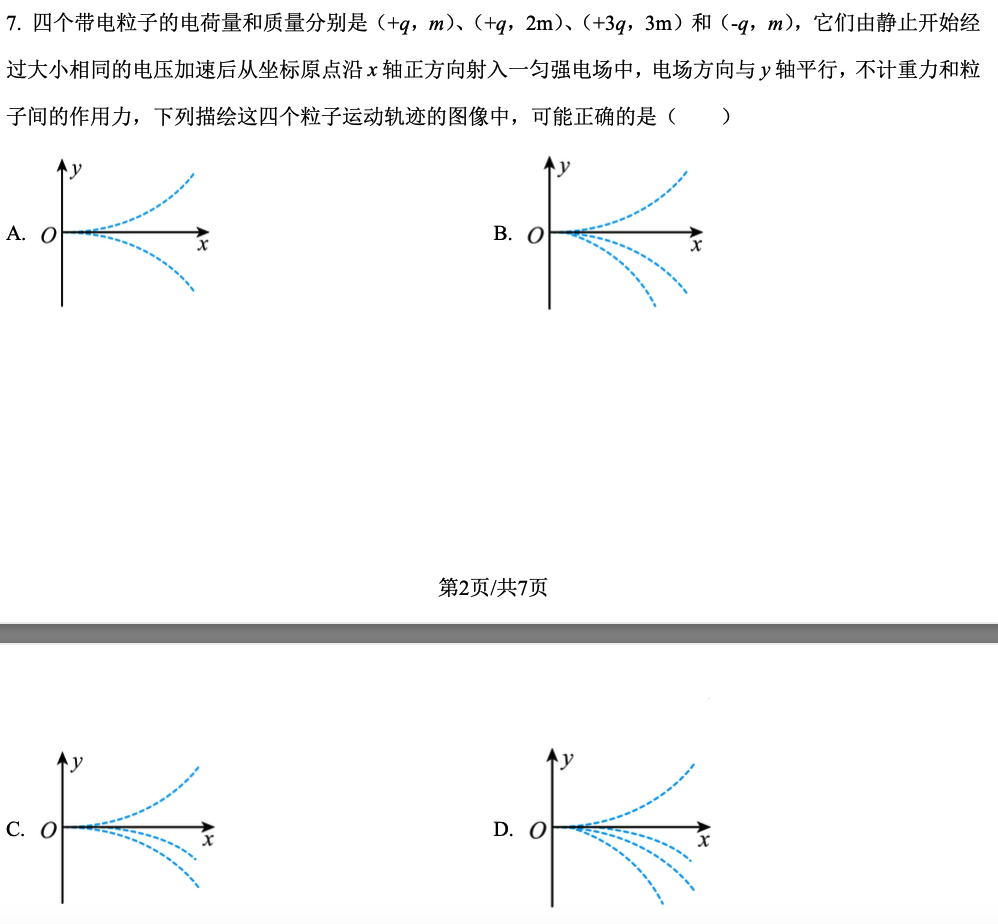
\includegraphics[width=50em,keepaspectratio]{./pictures/1.1-1.png}

    \begin{itemize}
        \item 错选:\quad B
        \item 正解:\quad A
        \item 总结:最终要给出\textbf{轨迹方程,即$ y = f(x) $},同时注意\textbf{电荷的正负性}决定着轨迹函数所在的区间
        \item 扩展:荷质比相关题目,粒子回旋加速期、粒子速度筛选器等
    \end{itemize}

    \subsubsection{II-9}
    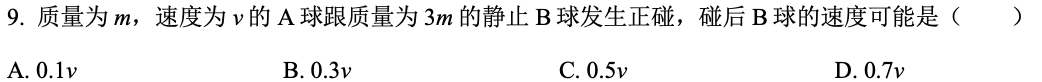
\includegraphics[width=50em,keepaspectratio]{./pictures/1.1-2.png}

    \begin{itemize}
        \item 错选:\quad ABC
        \item 正解:\quad BC    
        \item 总结:\quad 容易用不等式解法去求得$3m$物块的最大速度,但是无法计算最小速度。事实上$3m$物体碰
        后的\textbf{速度区间取决于碰撞过程中的动能损失程度}。
        \begin{itemize}
            \item \textbf{弹性碰撞(完全弹性碰撞)},系统机械能损失\textbf{最小},获得被碰物体\textbf{最大速度}
            \item \textbf{非弹性碰撞},系统机能损失,特点是碰后两物块\textbf{分离}
            \item \textbf{完全非弹性碰撞},碰撞后物体"粘连"  $ \lra mv_{0} = (m+3m)v^{'} $在一起,系统动能损失\textbf{最大},被碰物体获得\textbf{最小速度}。
        \end{itemize}
    \end{itemize}

    \subsubsection{II-10}
    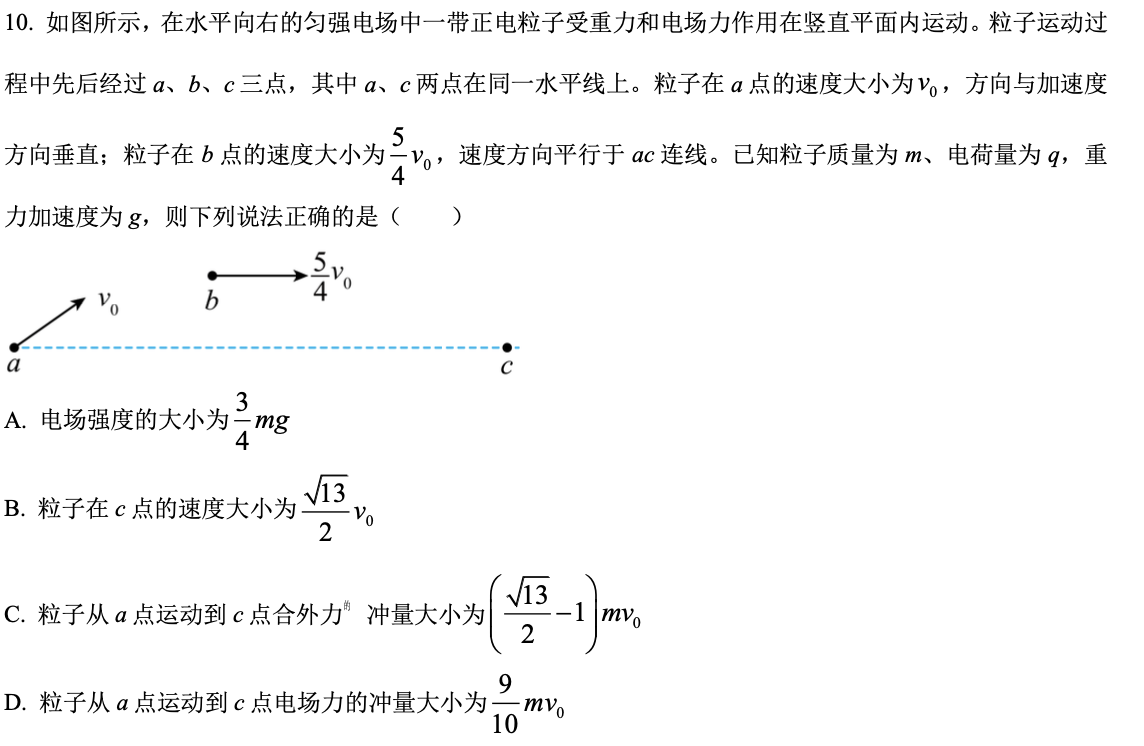
\includegraphics[width=50em,keepaspectratio]{./pictures/1.1-3.png}

    \begin{itemize}
        \item 正解:\quad BD
        \item 总结:\quad 
            \begin{itemize}
                \item 选项A \\
                        重点在于粒子在$a$点时的速度方向与加速度方向垂直。因此 \quad $b$点的速度在初速度方向的投影 \quad 与 \quad 初速度的大小一致。由此可以求得初始速度方向与水平方向的夹角$\theta$。再通过
                        相同时间内($a \rightarrow b$),重力冲量与电场力冲量下对两个方向的动量改变量,获得的两个方程消去时间$\triangle t$,得到$Eq$与$mg$的数量关系(选项$A$量纲错误)。
                        $$
                        \begin{cases}
                            mg \vdot \triangle t = m v_{0} \vdot \sin{\theta}           \\
                            Eq \vdot \triangle t = \frac{5}{4} m v_{0} - m v_{0} \vdot \cos{\theta}
                        \end{cases}
                        $$

                \item 选项B \\
                      在同一水平面上,$a \rightarrow c$的时间为$a \rightarrow b$的时间的两倍(竖直运动的对称性).
                      
                      \begin{align*}
                        mg \vdot t &= 2 m v_{0} \sin{\theta} \lra t = \frac{6 v_{0}}{5 g}    \\
                        m v_{x} - m v_{0} \cos{\theta} &= Eq \vdot t \quad (Eq = \frac{3}{4} mg)
                      \end{align*}
                      计算合速度可以先使用水平方向上的冲量定理计算出水平方向上的速度。或者直接用动能定理(重力势能不变),计算出$a \rightarrow c$的水平距离,进而得到电场力做功。
            \end{itemize}        
        \item 扩展:\quad
    \end{itemize}

    \subsubsection{III-1}
    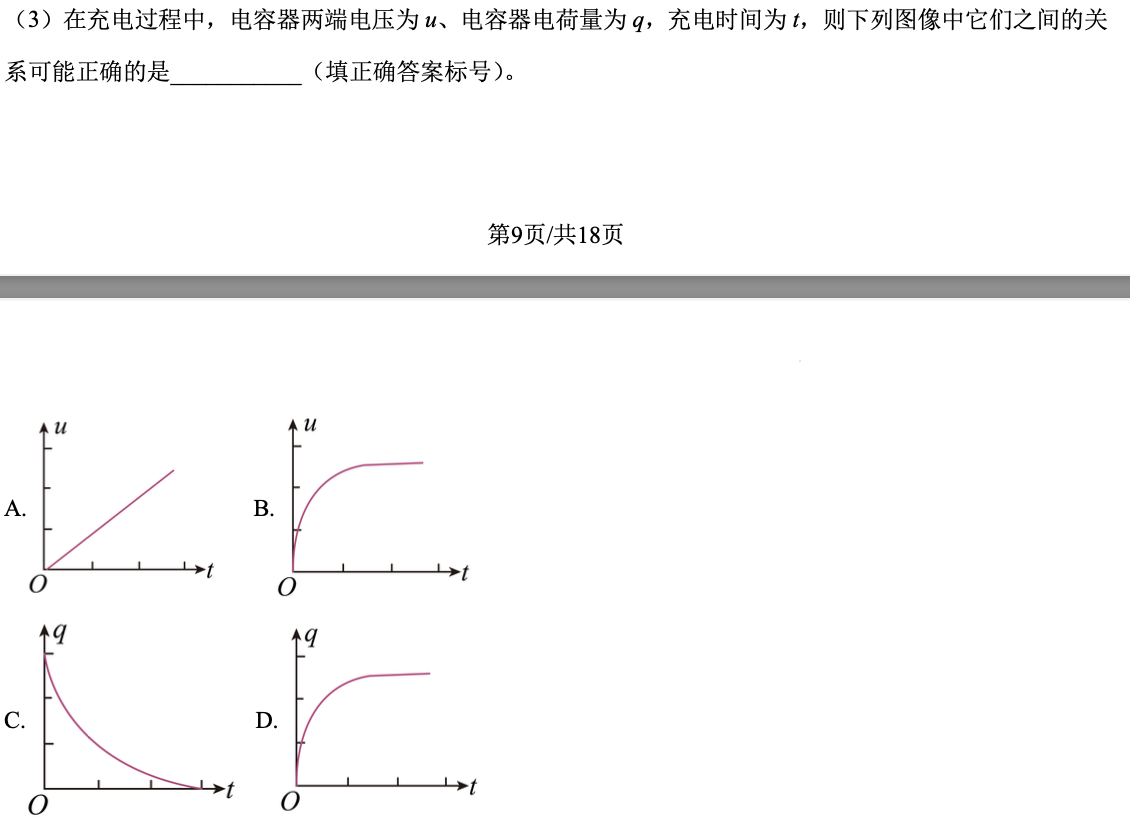
\includegraphics[width=50em,keepaspectratio]{./pictures/1.1-4.png}

    \begin{itemize}
        \item 错选:\quad D
        \item 正解:\quad BD
        \item 总结:\quad 电容器的电压并非在一瞬间就获得,同样是电荷累计的结果
    \end{itemize}


    \subsection{2022-2023育才中学期末模拟题(八)}

    \subsubsection{I-4}
    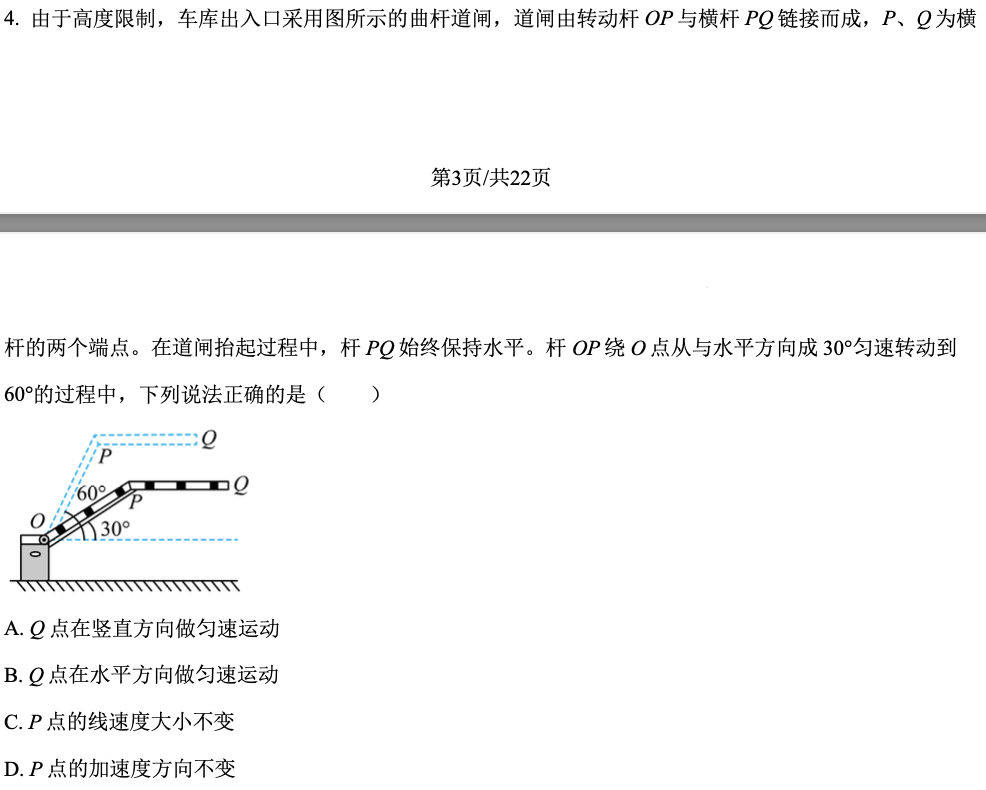
\includegraphics[width=50em,keepaspectratio]{./pictures/1.2-1.png}

    \begin{itemize}
        \item 正解:\quad C
        \item 总结:\quad 选出正确答案并不难,本质是$\omega_{//}$
        \item 扩展:\quad 进一步思考本题,$P$点的运动为匀速圆周运动,因此其坐标$(x,y)$是可以被表示的.
                  $$
                  P_(x,y) = (\cos{(\omega t + \phi_{0})} , \sin{(\omega t + \phi_{0})})
                  $$
                  同时$Q$点的坐标也是可以被表示的,存在\textbf{几何约束},$P$到$Q$的距离为固定值线段$\overline{PQ} = L$,显然$Q$也是做匀速圆周运动
                  圆心为距离圆心$O$右侧$L$处,且角速度小于$P$点.
    \end{itemize}
 
    \subsubsection{I-7}
    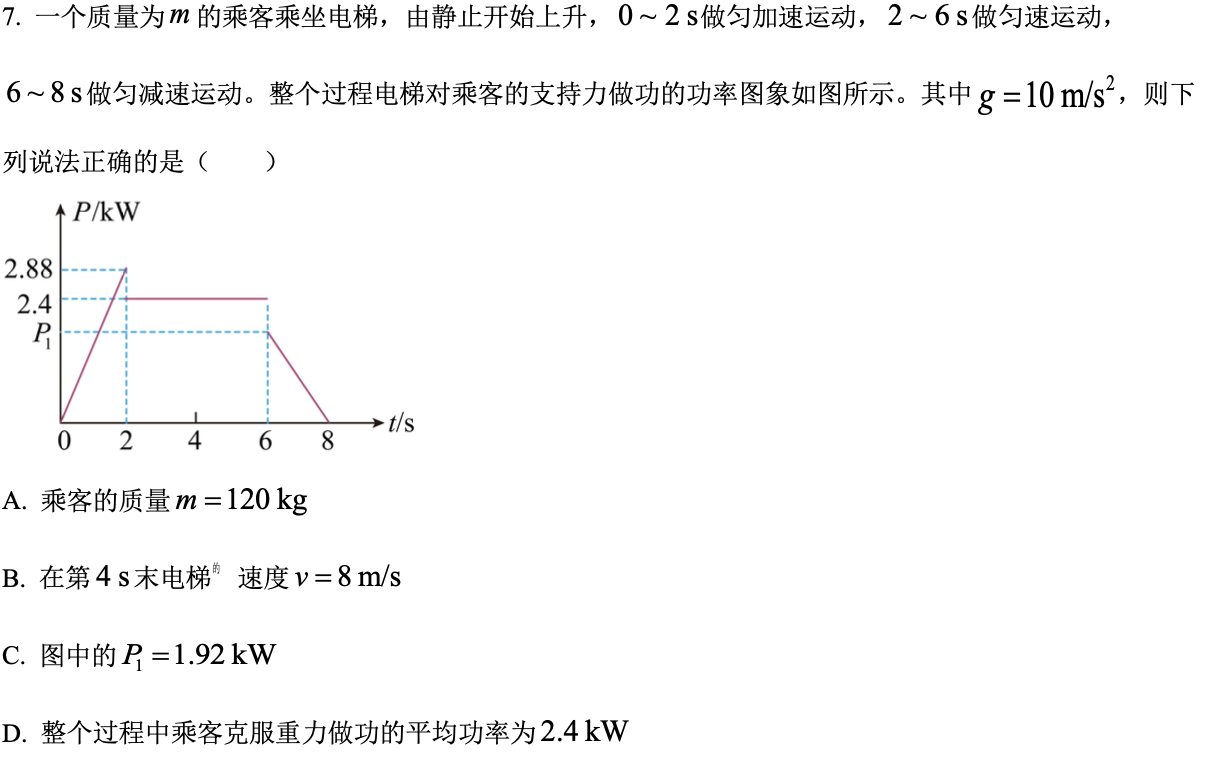
\includegraphics[width=50em,keepaspectratio]{./pictures/1.2-2.png}

    \begin{itemize}
        \item 正解:\quad C
        \item 总结:\quad 此题分为三个阶段,同时存在一个重要的速度节点,即$t = 2s$时的速度.所列方程众多,因此理清阶段,以及要求的目标量.
                  $$
                  \begin{cases}
                    P_{1} = N \vdot a \vdot t = 2880 w  \\
                    P_{2} = mg \vdot a \vdot t  = 2400 w
                  \end{cases}
                  $$
                  选项$D$,可以有两种思路;第一种:计算出位移,得到重力势能做功.第二种$P-t$图所围成的面积为支持力做功的平均功率,在此过程中无
                  其他力做功且初末动能均为0,因此支持力做功的平均功率等于克服重力做功的平均功率.
                  $$ W = 1920j + 2880j + 9600 j \qquad t_{total} = 8s \qquad \overline{P} = \frac{W}{t_{total}} = 1.8kw $$

        \item 扩展:
            \begin{align}
            P &= N \vdot v \qquad v = v_{0} + a t \qquad v_{0} = 0 \qquad a = \frac{N-mg}{m} \\
            P &= \frac{N(N-mg)}{m} t \qquad  k = \frac{N(N-mg)}{m}
          \end{align}
    \end{itemize}
    
    \subsubsection{II-8}
    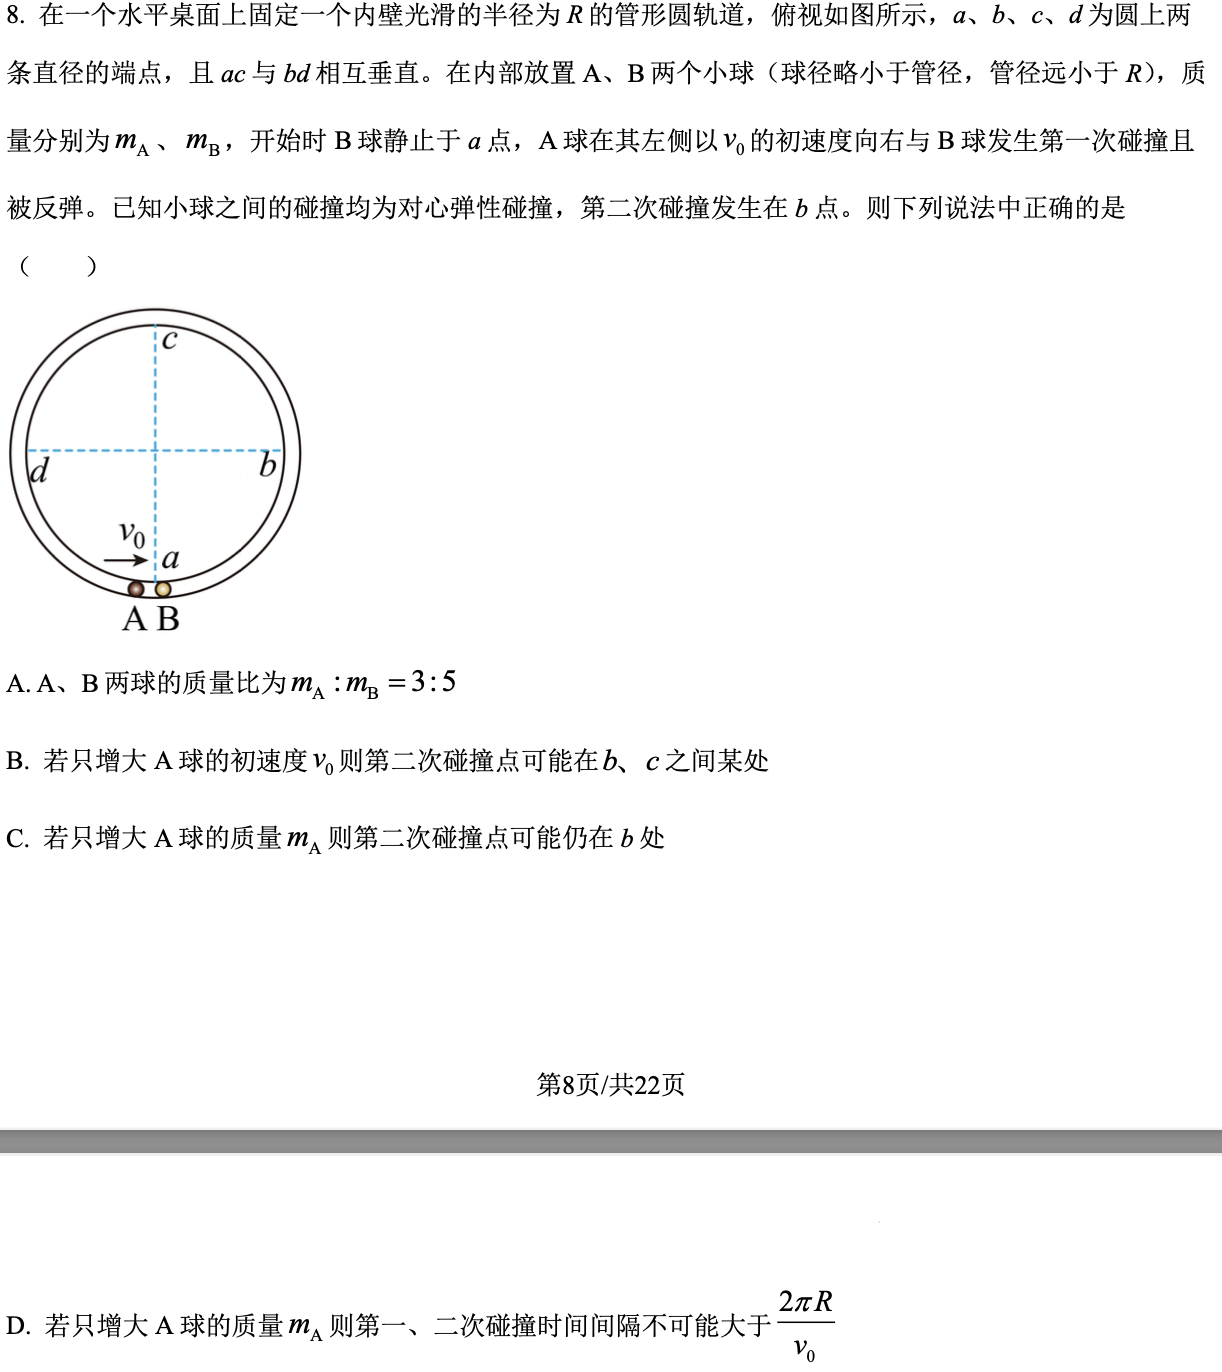
\includegraphics[width=50em,keepaspectratio]{./pictures/1.2-3.png}

    \begin{itemize}
        \item 错选:\quad
        \item 正解:\quad CD
        \item 总结:\quad 此物理情景发生在水平桌面上,所以不用考虑重力.所以本质是一个追及问题。同时第二次碰撞满足三个方程,第一个方程控制碰撞约束,第二、三个方程控制具体
                  碰撞点
                  $$
                  \begin{cases}
                    v_{A} t + v_{B} t = 2 \pi R     \\
                    v_{B} t  = \frac{\pi}{2}        \\
                    v_{A} t = \frac{3\pi}{2}
                  \end{cases}
                  $$
                  选项$B$,通过前面的计算碰撞发生的时间为$t = \frac{2\pi R}{v_{0}}$ 仅仅与$v_{0}$有关,但碰后的速度也发生了变化,因此我们需要设出
                  碰撞时的角度(这里取与水平线上为$\alpha$),计算出该角度的函数表达式(关于初速度质量等)
                  $$
                  \begin{cases}
                    v_{A} t &= (\frac{3\pi}{2} - \alpha) R \\
                    v_{B} t &= (\frac{\pi}{2} + \alpha) R  \\
                    v_{A} &= \frac{m_{B} - m{A}}{m_{A}+m{B}} v_{0}   \\
                    v_{B} &= \frac{2 m{A}}{m_{A}+m{B}} v_{0} 
                  \end{cases}   
                  $$

                  $$
                  \alpha = \frac{7 \pi}{2} \vdot \frac{m_{A} - m_{B}}{m_{A} + m_{B}} 
                  $$
                  其碰撞点与初速度无关所以$B$错,与质量相关,当碰撞点在$b$时存在球$A$反向碰撞(题目初始情况)与球$A$同向被套圈碰撞,所以$C$对,满足$m_{A} : m_{B} = 5 : 3$
    \end{itemize}

    \subsubsection{III-12}
    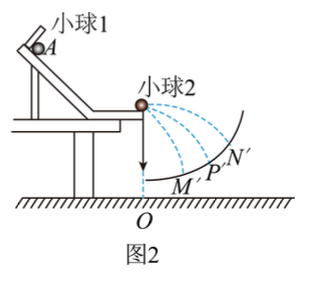
\includegraphics[width=10em,keepaspectratio]{./pictures/1.2-4.png}
    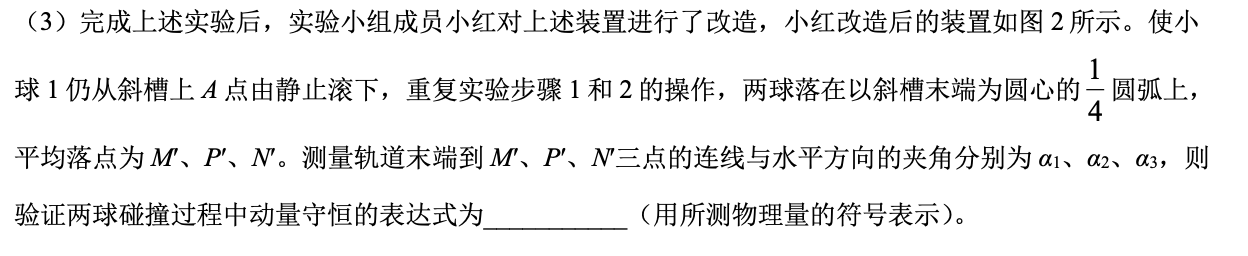
\includegraphics[width=40em,keepaspectratio]{./pictures/1.2-5.png}

    \begin{itemize}
        \item 总结:夹角$\alpha$为位移偏转角.这类题目已知位移偏转角同时还有几何约束那么易得
        $$
        \begin{cases}
            x = R \cos{\alpha} = v_{x} t \\
            y = R \sin{\alpha} = \frac{1}{2} g t^{2} \\
        \end{cases}
        $$

        $$
        \lra v_{x} = \sqrt{\frac{gR}{2}} \vdot \sqrt{\frac{\cos^{2}{\alpha}}{\sin{\alpha}}} \quad  \llra \quad  v_{x}  \propto  \sqrt{\frac{\cos^{2}{\alpha}}{\sin{\alpha}}}
        $$

    \end{itemize}

    \subsubsection{IV-2}
    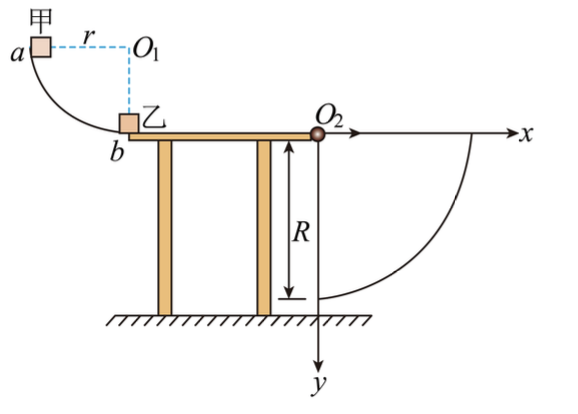
\includegraphics[width=50em,keepaspectratio]{./pictures/1.2-6.png} \\
    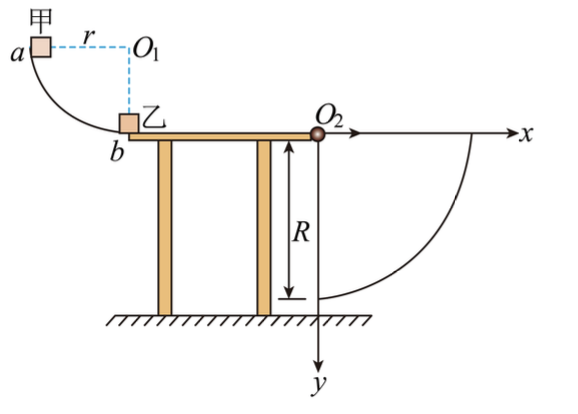
\includegraphics[width=20em,keepaspectratio]{./pictures/1.2-7.png}

    \begin{itemize}
        \item 总结:\quad 在解方程组的时候,选择去消掉$t$直接得到$v = f(v_{0})$是非常困难的,事实上先解出$v = f(y)$求得最小的
                  $y_{min}$,那么就可得到最小的$v_{ymin}$进而得到最小的$v = \sqrt{gh}$
    \end{itemize}
    

    \subsection{2022-2023巴蜀中学下学期期末}
    \subsubsection{I-13}
    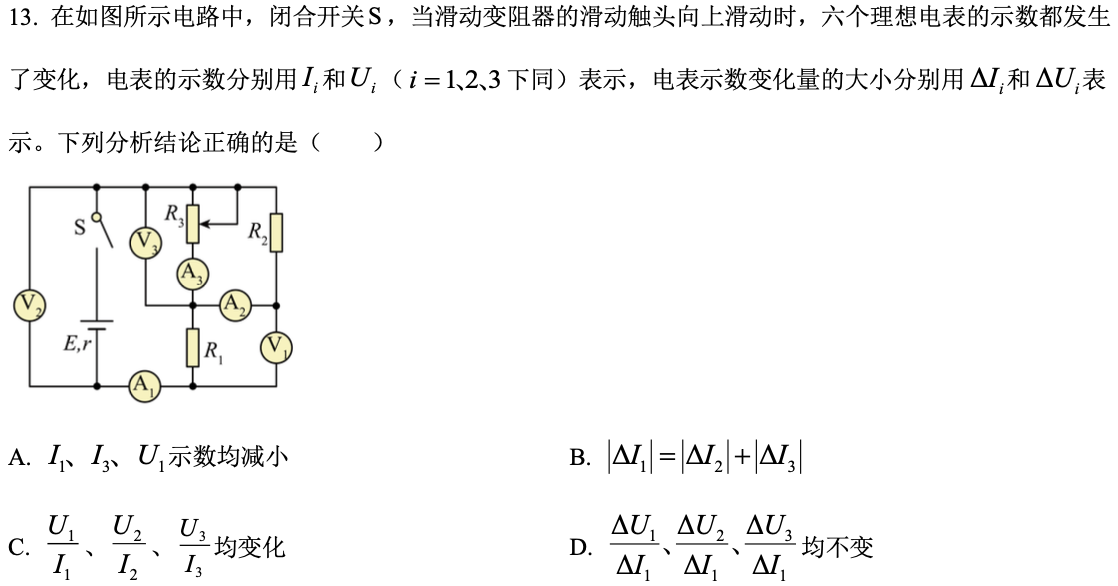
\includegraphics[width=50em,keepaspectratio]{./pictures/1.2-8.png}

    \begin{itemize}
        \item 总结: \quad 最好写出回路的表达式$E = U_{2} + I_{1}r  \quad U_{3} = E - I_{1}(R_{1} + r)$ 
    \end{itemize}

    \subsubsection{II-2}
    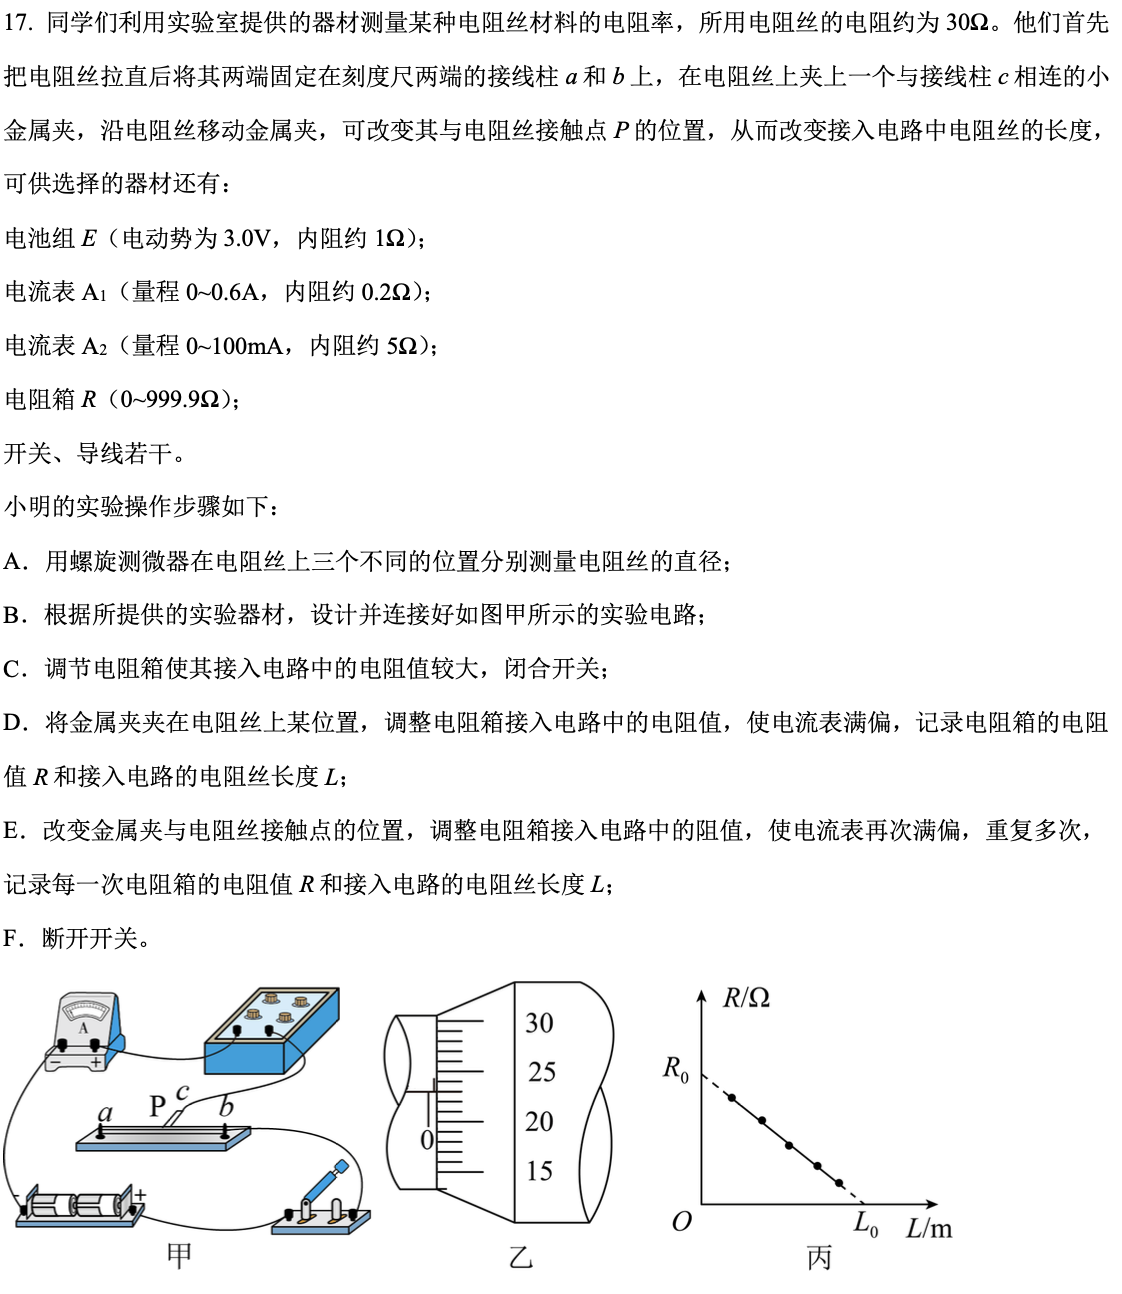
\includegraphics[width=50em,keepaspectratio]{./pictures/1.2-9.png}  \\
    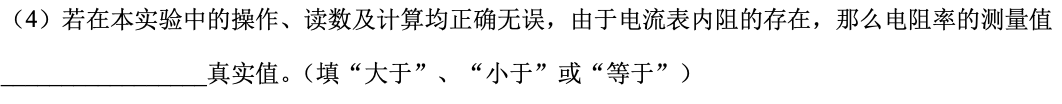
\includegraphics[width=50em,keepaspectratio]{./pictures/1.2-10.png}

    \begin{itemize}
        \item 总结:\quad 官解结果正确但是思路奇怪,$R_{0}$会发生变化,存在电流表内阻时
              $$
              R_{0} = \frac{E}{I} - r
              $$
              所以$R_{0}$测量值偏小,但事实上实验步骤并不直接得到$R_{0}$,而是通过延长线的方式,因此$L_{0}$并非不变化的

              $$
              R_{i} = \frac{E}{I_{满偏}} - r -\frac{4\rho}{\pi d^{2}} L_{i}
              $$

              实验的测量值是准确的,因此忽略电流表内阻与仅仅是将直线向下移动,并不影响斜率,所以结果是等于
    \end{itemize}

    \subsection{2023届巴蜀中学高考适应性月考(十)}
    \subsubsection{I-6}
    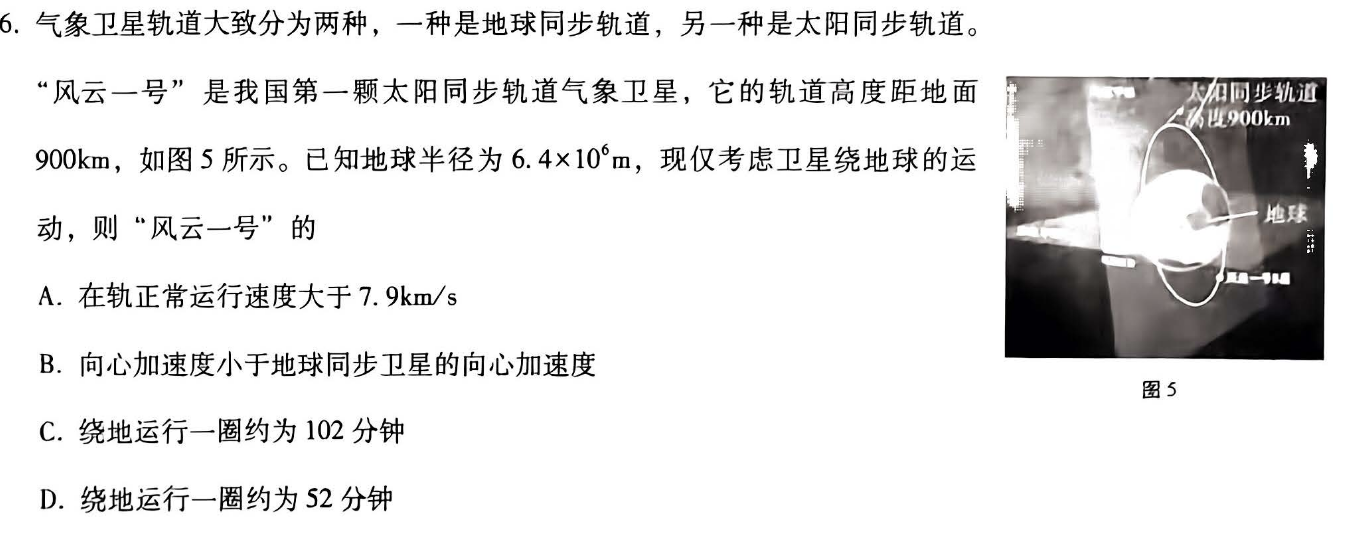
\includegraphics[width=50em,keepaspectratio]{./pictures/1.3-1.png}

    \begin{itemize}
        \item 正解:\quad C
        \item 总结:\quad 
        \begin{itemize}
            \item 近地卫星:其\textbf{运动轨道半径约为地球半径},因此为\textbf{最大的环绕速度$7.9km/s$},周期为85分钟(不用记忆)
            \item 同步卫星:其\textbf{周期与地球自转相同为$24h$}
        \end{itemize}
        \item 扩展:第三与四个选项的计算需要知道两个竖数值中的一个
            \begin{itemize}
                \item 同步卫星的轨道高度为$3.6 \cross 10^{7} m$,然后用开普勒第三定律
                \begin{thm*}
                    开普勒行星运动定律(不用纠结证明)
                    \begin{itemize}
                        \item 第一定律:行星运动在椭圆轨道上,太阳处于椭圆的焦点上
                        \item 第二定律:行星与太阳的连线在相同时间内扫过的面积相等
                        \item 第三定律:$\frac{a^{3}}{T^{2}} = k$
                    \end{itemize}
                \end{thm*}
                \item 近地卫星的周期为$85$分钟,根据第三定律得知太阳同步轨道卫星的周期至少大$85$分钟,因此选$C$
            \end{itemize}
    \end{itemize}

    \subsubsection{II-1}
    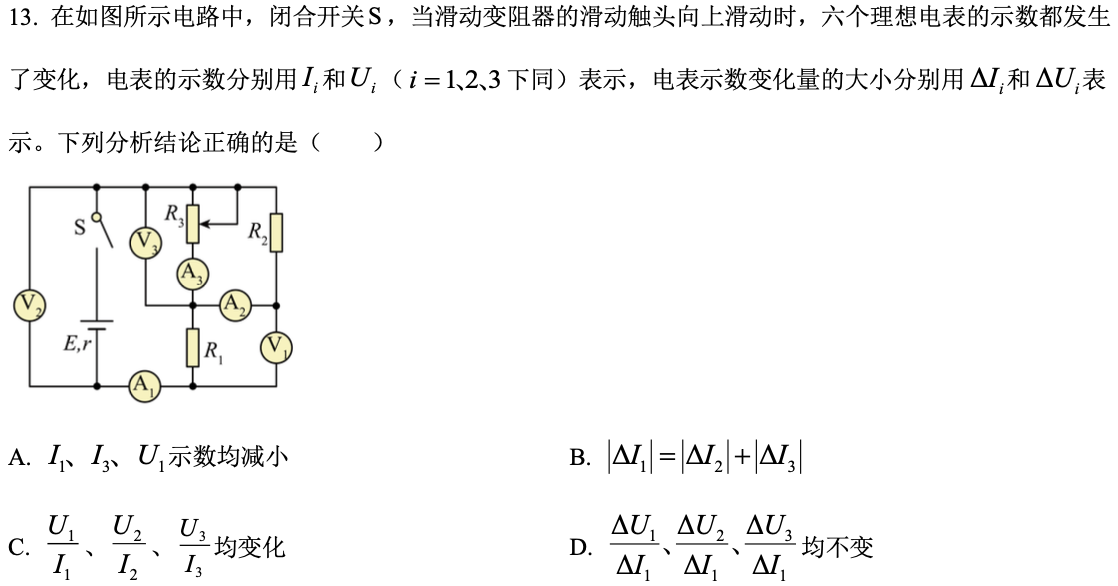
\includegraphics[width=50em,keepaspectratio]{./pictures/1.3-2.png}

    \begin{itemize}
        \item 错选:\quad BC
        \item 正解:\quad BD
        \item 总结:\quad 选项$C$问的是起振($t=0s$)方向,而题目\textbf{图乙}是给的$t=1s$的质点振动图\\
                        选项$D$需要求$t=\frac{1}{3}s$时对应的$y$值,所以需要根据图像中已知数据点求解三角函数的具体表达式
    \end{itemize}

        \begin{proof}
            设$ y = 10 \sin{\omega t + \phi_{0}}$
            \begin{align*}
                t &= 0s \quad \sin{\phi_{0}} = 0 \lra \phi_{0} = 0   \\
                t &= 1s \quad \sin{\omega} = 0 \lra \omega = n\pi    \\
                t &= \frac{1}{2}s \quad \sin{\frac{\omega}{2}} = 1 \lra \omega = \pi + 4n\pi
            \end{align*}
        \end{proof}
        $$
        y = 10\sin{\pi t} \quad t = \frac{1}{3}s \lra y = 10 \vdot \frac{\sqrt{3}}{2} = 5\sqrt{3}
        $$
    
    \subsubsection{II-3}
    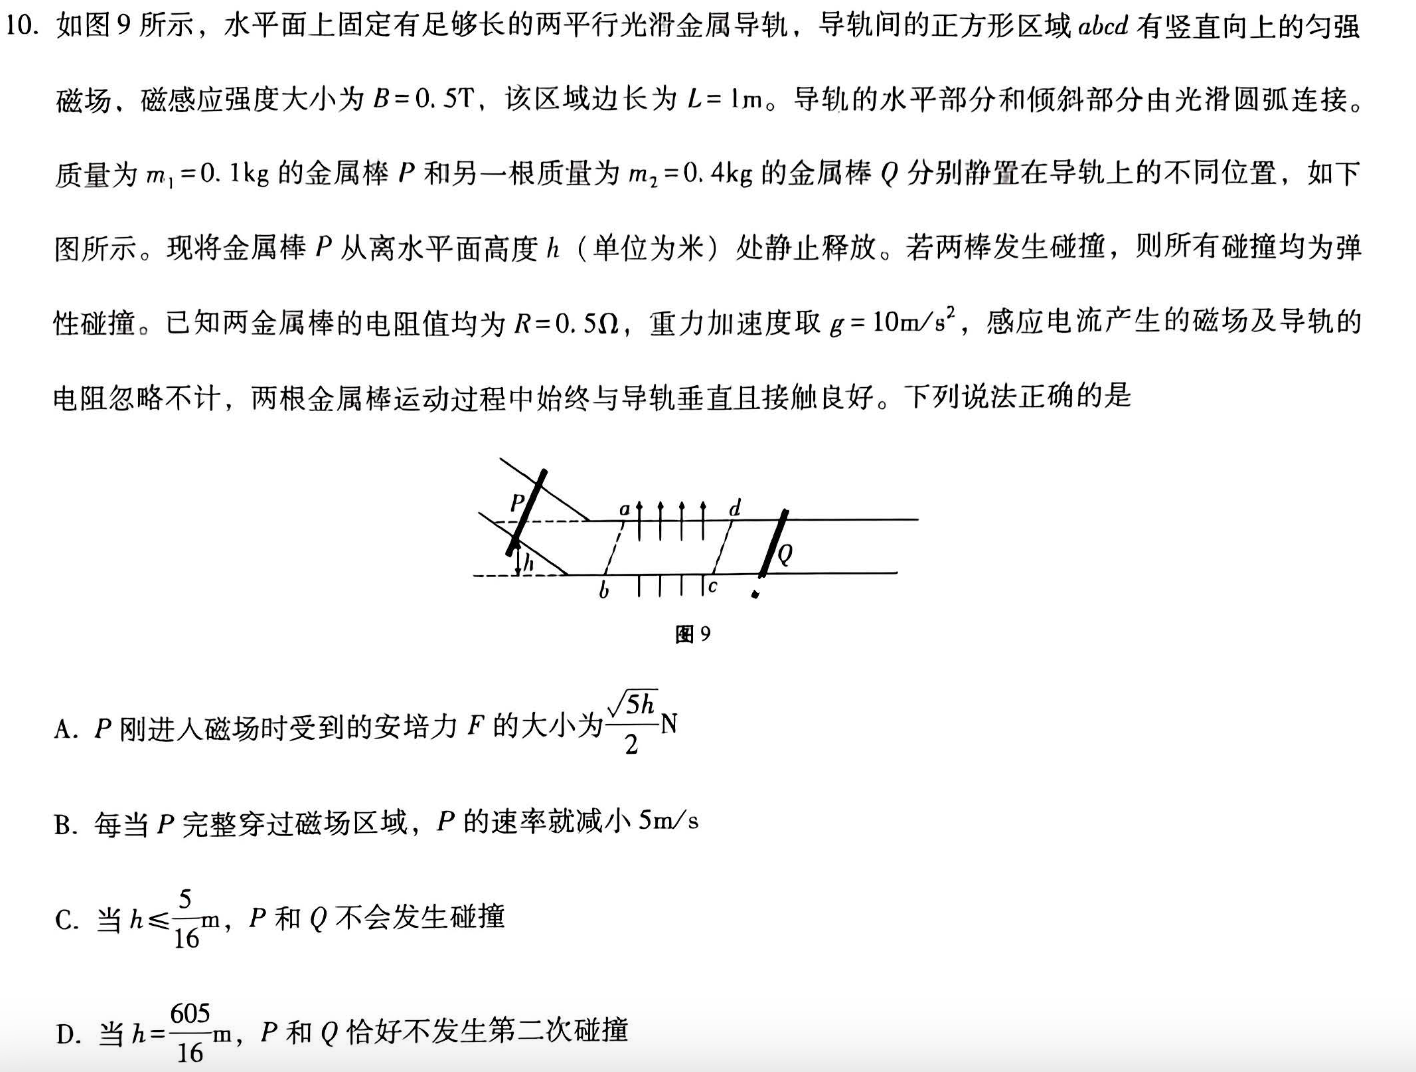
\includegraphics[width=50em,keepaspectratio]{./pictures/1.3-3.png}

    \begin{itemize}
        \item 错选:\quad AC
        \item 正解:\quad ACD
        \item 总结:\quad 选项B, $E = - \frac{\triangle \Phi}{\triangle t}$,在高中阶段$\triangle t$比较小的时候为瞬时
        电动势,当$\triangle t$比较大的时候,即为一个过程量得到的是$\overline{E}$,因此可以得到$\overline{I},\overline{F}$
        \begin{align*}
            \varepsilon &= \frac{\triangle \Phi}{\triangle t} = \frac{B \vdot \triangle S}{\triangle t}   \\
            I &= \frac{\varepsilon}{2R} = \frac{B}{2R} \vdot \frac{\triangle S}{\triangle t} \\
            F &= B I L = \frac{B^{2}L \triangle S}{2R \vdot \triangle t}    \\
            F \vdot \triangle t &= \frac{B^{2} L \triangle S}{2 R} = m(v_{t} - v_{0})
        \end{align*}
        复杂变化的安培力对导体棒的冲量,仅仅与面积的改变量有关$\lra$速度的变化量仅与走过的面积有关 \\
        选项D,恰好不能第二次碰撞即再次扫过2次磁场面积后速度为球2第一次碰后速度
    \end{itemize}
    
    \subsubsection{IV-1}
    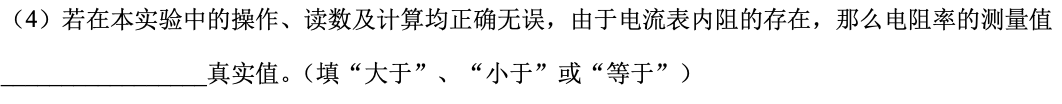
\includegraphics[width=50em,keepaspectratio]{./pictures/1.3-4.png}

    \begin{itemize}
        \item 总结:好题收藏,第二问关键在与「沙粒随时间均匀漏下」,从已知条件中求出\textbf{沙粒平均流量},计算第二段的时间长度即可
    \end{itemize}

    
    \subsubsection{IV-2}
    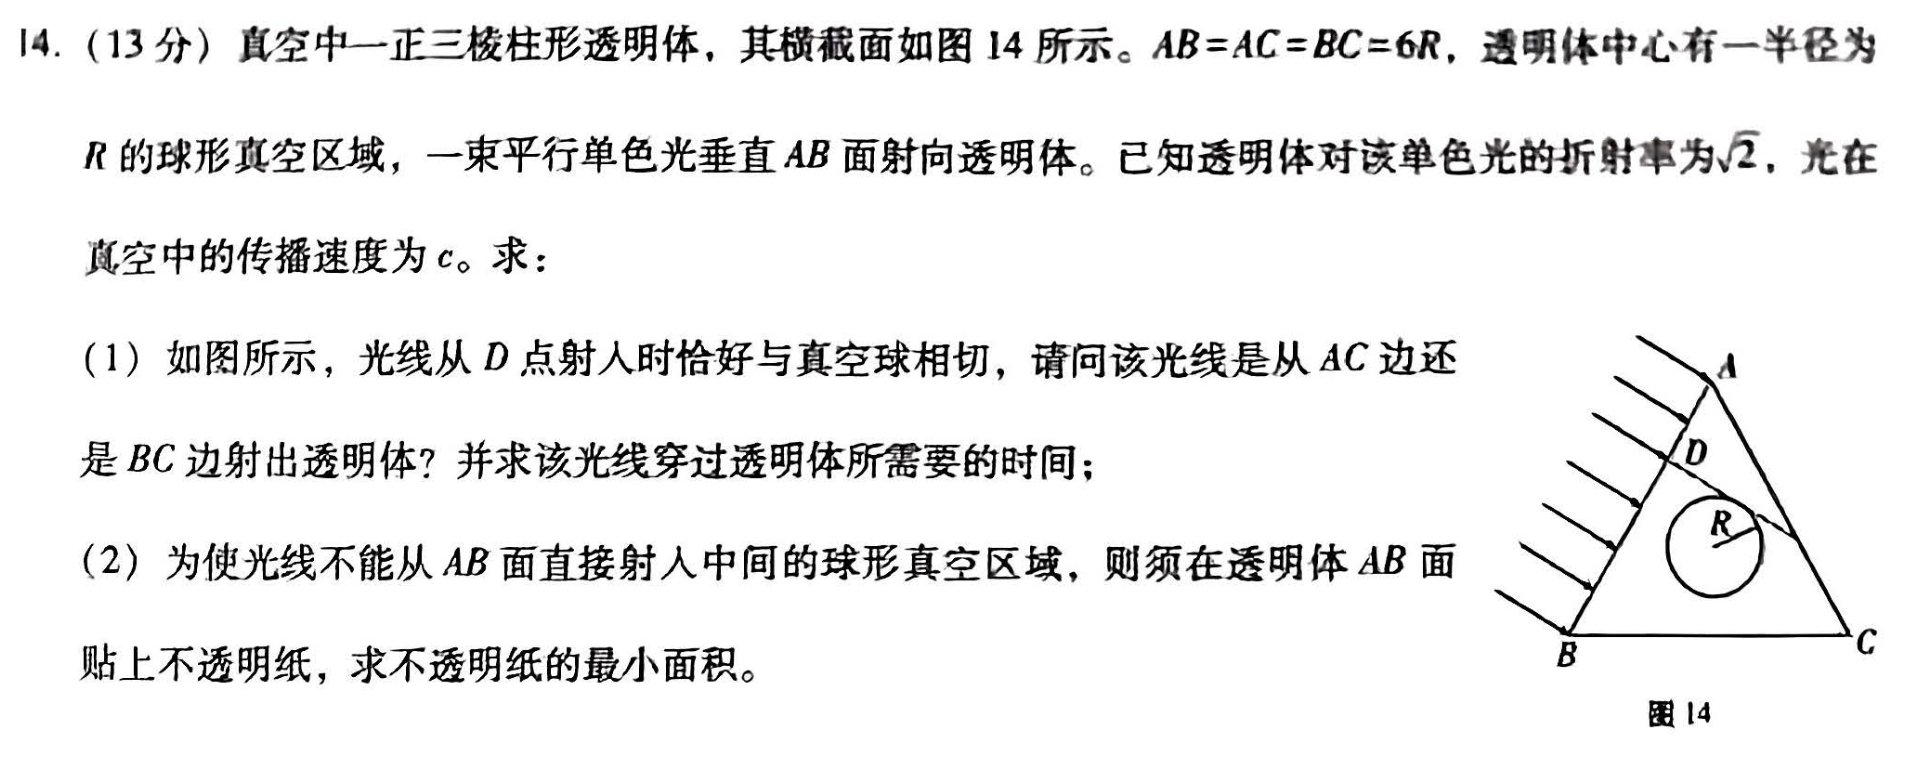
\includegraphics[width=50em,keepaspectratio]{./pictures/1.3-5.png}
    
    \begin{itemize}
        \item 总结:第一问当光垂直入射介面交界处 or 平行入射介面交界处,光路沿原方向继续传播
        \item 第二问不难,即光线接触真空区域时,以临界角$\frac{\pi}{2}$射入,值的思考的是遮挡面积是一个圆形域
    \end{itemize}

        
    \subsubsection{IV-3}
    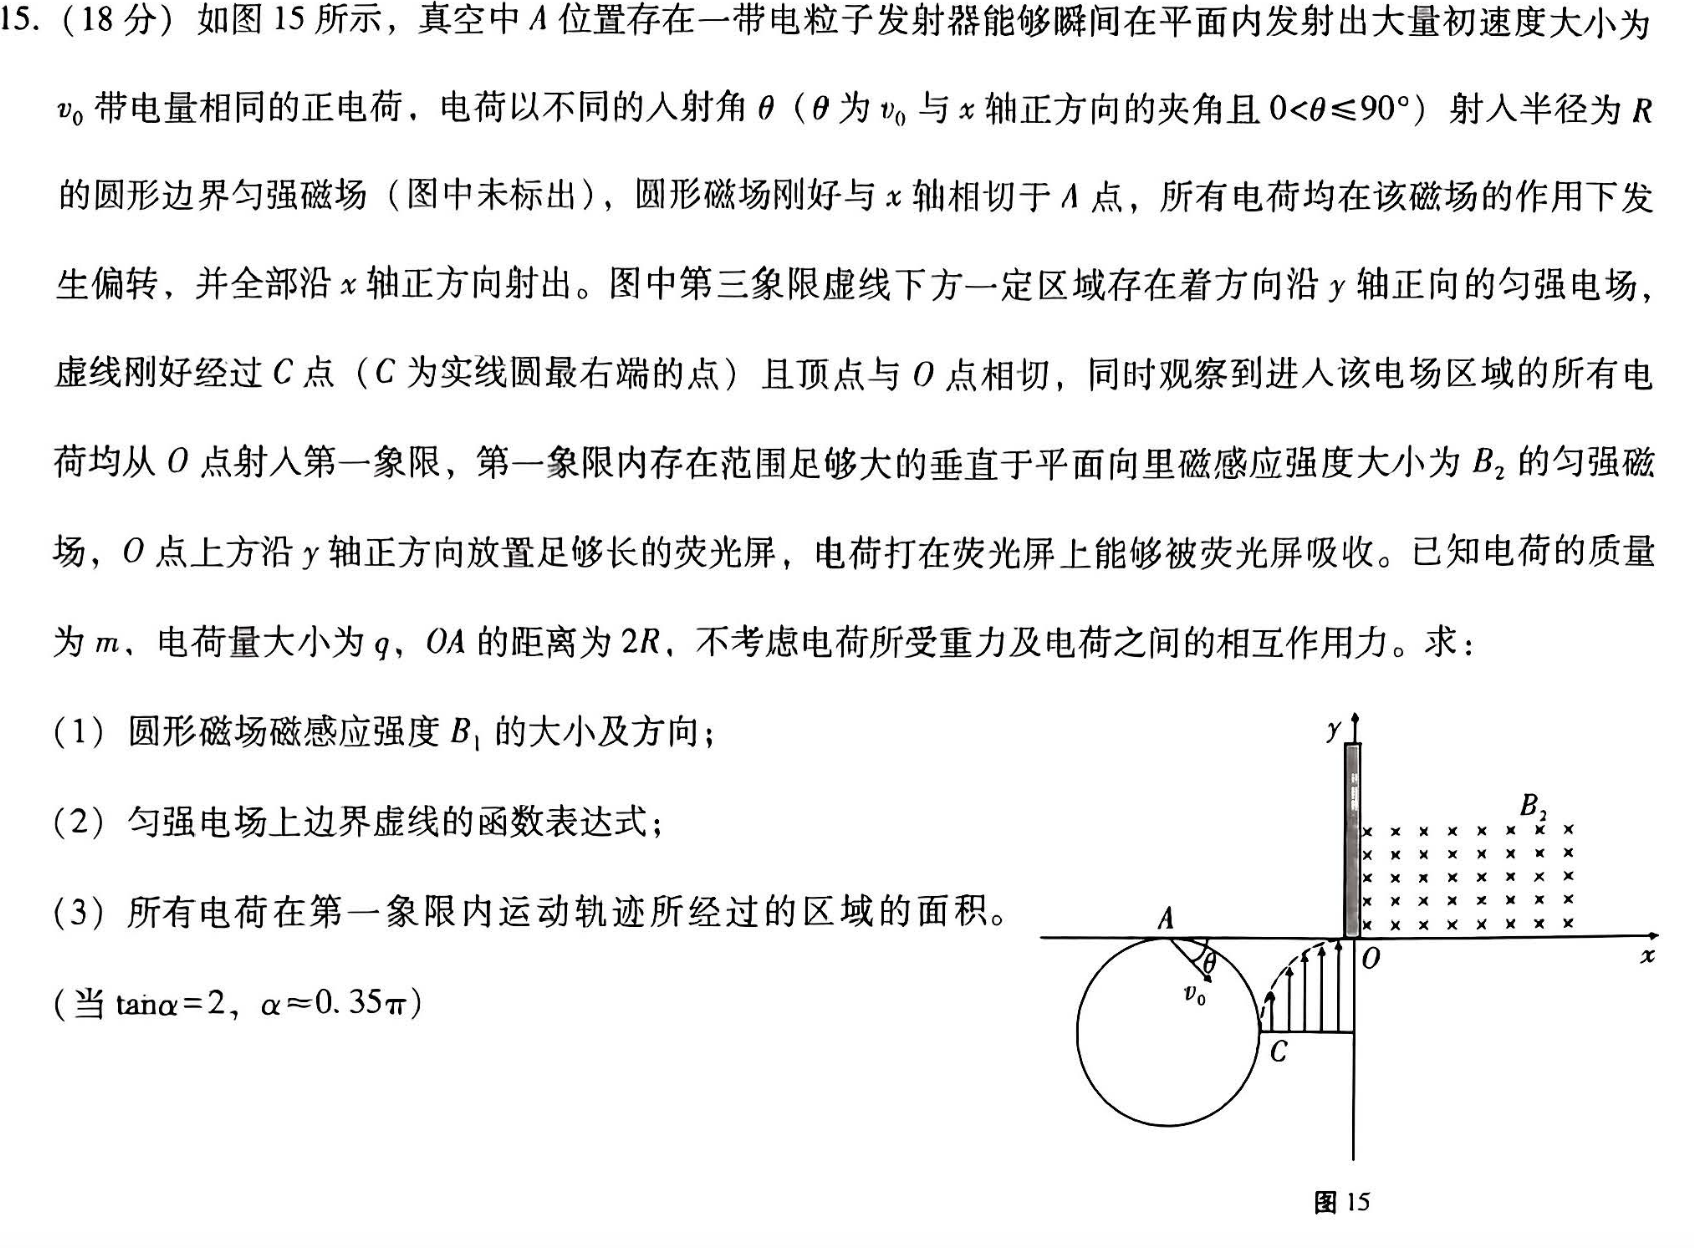
\includegraphics[width=50em,keepaspectratio]{./pictures/1.3-6.png}

    \begin{itemize}
        \item 总结:\quad 第一问考的\textbf{磁聚焦}(证明通过相似三角形),粒子旋转半径刚好为磁场半径$R$,也可以取特殊角度$\frac{\pi}{2}$
        \begin{figure}[h]
            \centering
            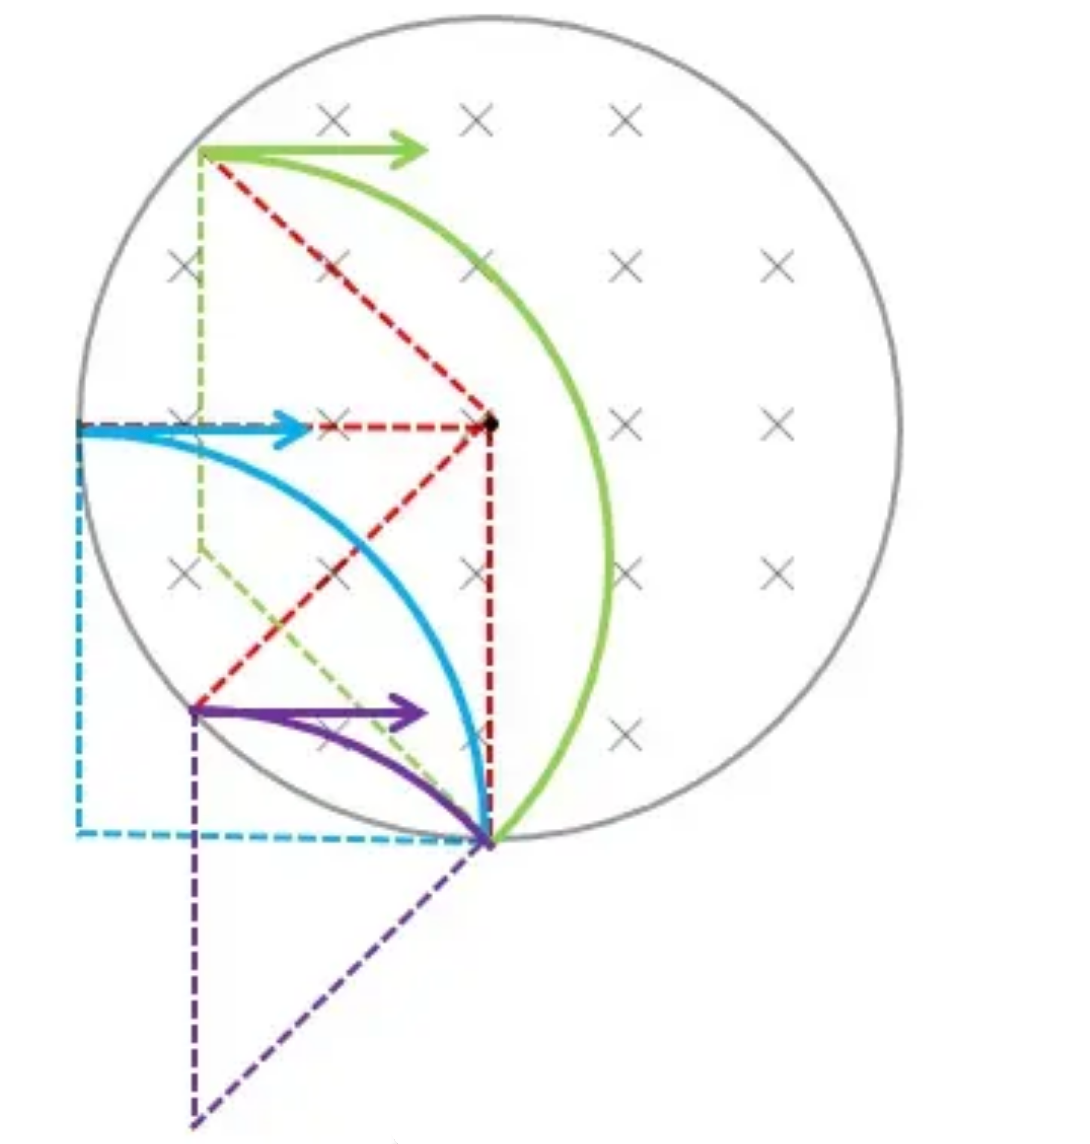
\includegraphics[width=20em,keepaspectratio]{./pictures/1.3-7.png}
        \end{figure}
        \item 第二问不难,注意电场需要求出来,设射入电场的粒子$(x_{0},y_{0})$,位移为坐标的负数.$E = \frac{2mv^{2}}{qR} \quad y = - \frac{1}{R} x^{2}$
        \item 第三问比较特殊,需要设$h$(距离下$x$轴的距离),去求不同高度下打到$y$轴上点的坐标,设进入第二磁场区域的速度方向与$x$轴成$\theta$角,打击点$ y = 2 r \cos{\theta}$
        $$
        \cos{\theta} = \frac{1}{\sqrt{1 + \frac{4h}{R}}} = 1 \quad \quad \quad r = \frac{mv}{qB_{2}} = \frac{mv_{0} \sqrt{1+\frac{4h}{R}}}{q B_{2}} = \frac{mv_{0} k}{qB_{2}}
        $$
        $$
        2 r \cos{\theta} = \frac{2mv_{0}}{qB_{2}}
        $$
        因此不同速度的粒子打在$y$轴上的点为同一点
        $$
        h = 0 \lra r_{0} = \frac{mv_{0}}{qB_{2}} \quad \quad \quad h = R \lra r_{1} = \frac{\sqrt{5} m v_{0}}{qB_{2}} \quad \theta = 0.35\pi
        $$
        \begin{align*}
            S_{0} &= \frac{1}{2} \vdot \pi r_{0}^{2} = \frac{\pi}{2} \vdot (\frac{mv_{0}}{qB_{2}})^{2} \\
            S{1} &= \pi r_{1}^{2} (\frac{\pi - 2\theta}{2 \pi}) - r_{1}^{2} \sin{\theta} \cos{\theta} = (\frac{3\pi}{4} - 2) \vdot (\frac{m v_{0}}{qB_{2}})^{2} \\
            S &= S_{0} - S_{1} = (\frac{8-\pi}{4}) \vdot (\frac{m v_{0}}{qB_{2}})^{2}
        \end{align*}
    \end{itemize}
        

        \subsection{2022-2023南开中学高一下期末}
        \subsubsection{I-6}
        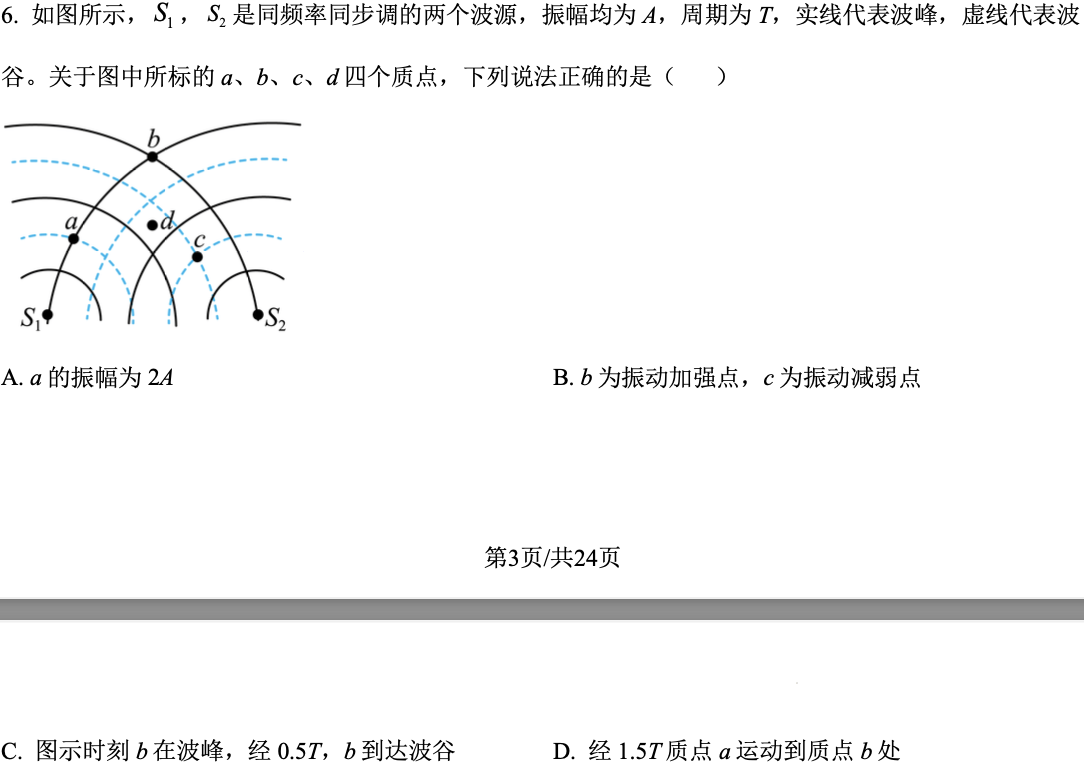
\includegraphics[width=50em,keepaspectratio]{./pictures/1.3-8.png}
        \begin{itemize}
            \item 正解:\quad C
            \item 总结:\quad 此为光波的另一种表现方式,同时\textbf{振动加强点包括波峰叠加和波谷叠加},D选项,质点$a$实际仅在平衡位置振动,并不产生其它方向的位移
        \end{itemize}

        \subsubsection{I-8}
        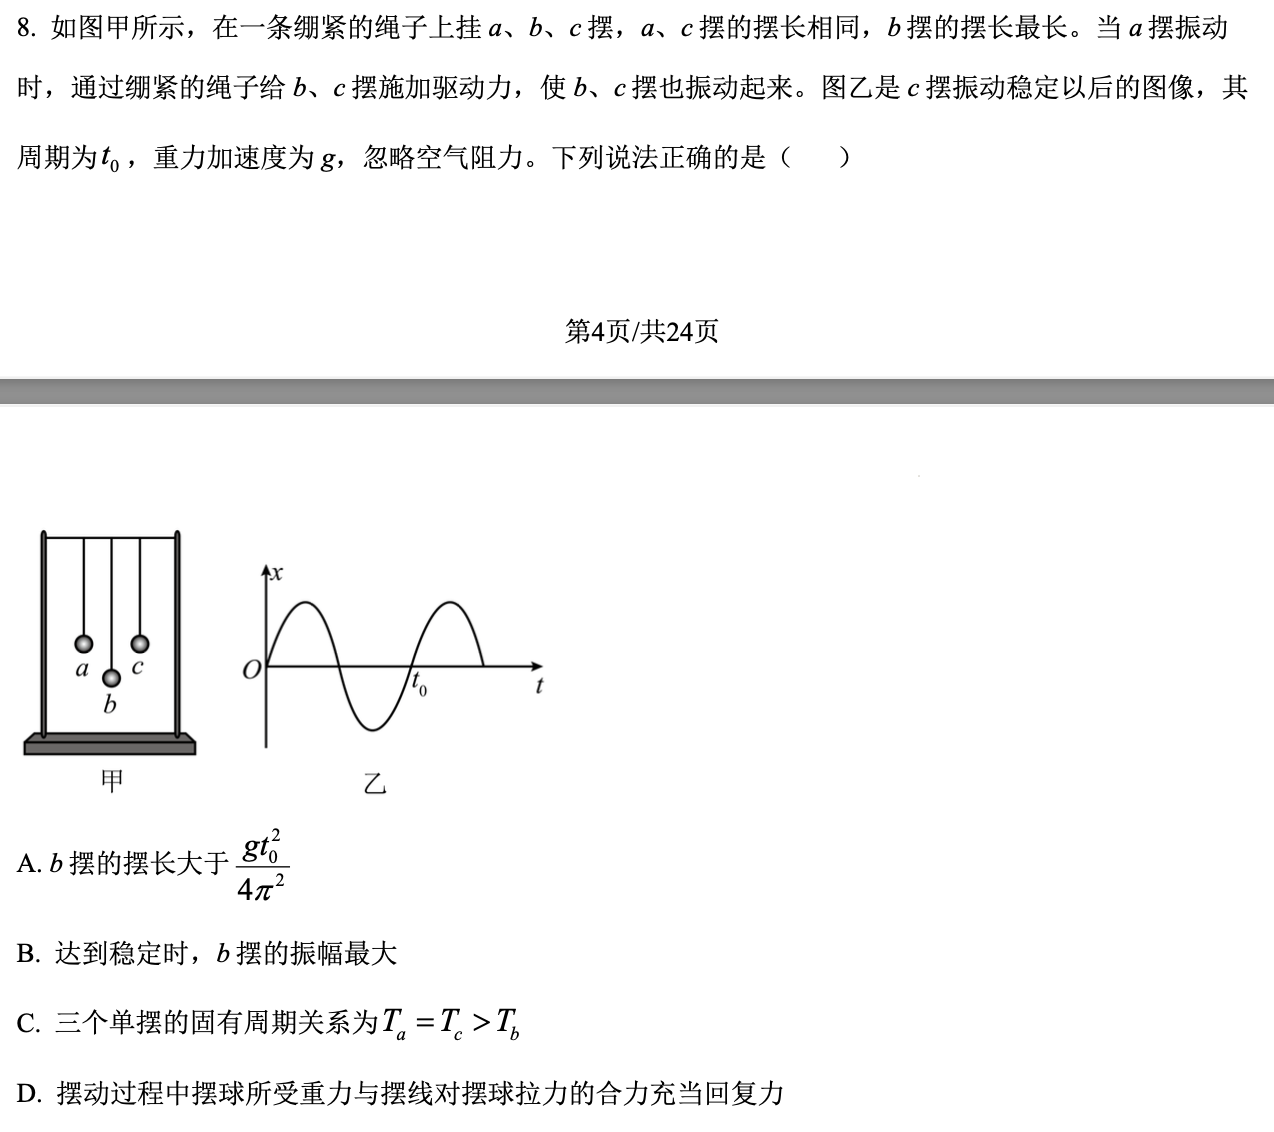
\includegraphics[width=50em,keepaspectratio]{./pictures/1.3-9.png}
        \begin{itemize}
            \item 正解:\quad A
            \item 总结:\quad 单摆周期公式死记硬背,受迫振动:在周期性外力的持续作用下而进行的振动称为\textbf{受迫振动},振动稳定后齐\textbf{频率}等于外力驱动频率
            $$
            T = 2 \pi \sqrt{\frac{L}{g}}
            $$
            \begin{proof}
                证明运动为简谐运动,仅需证明回复力$F = -kx$(多次进行小量近似,很简单)\\
            \end{proof}

            \begin{proof}
                证明简谐运动的周期(更复杂的方法请参考朗道等高阶解法)
                \begin{align*}
                    F = -\frac{mg}{L} \vdot x &= m \dv[2]{x}{t} \\
                    \dv[2]{x}{t} + \frac{g}{L}x &= 0 \\
                    \text{令} \quad \omega &= \sqrt{\frac{g}{L}} \\
                    \dv[2]{x}{t} + \omega^{2}x &= 0 \\
                    \text{特征根方程} \quad r^{2} = \omega^{2} \quad r &= \pm \omega i  \\
                    x = C \sin{(\omega t + \phi)} \quad \lra \quad T = \frac{2 \pi}{\omega} &= 2 \pi \sqrt{\frac{L}{g}}
                \end{align*}
            \end{proof}
        \end{itemize}

        \begin{figure}[h]
            \centering
            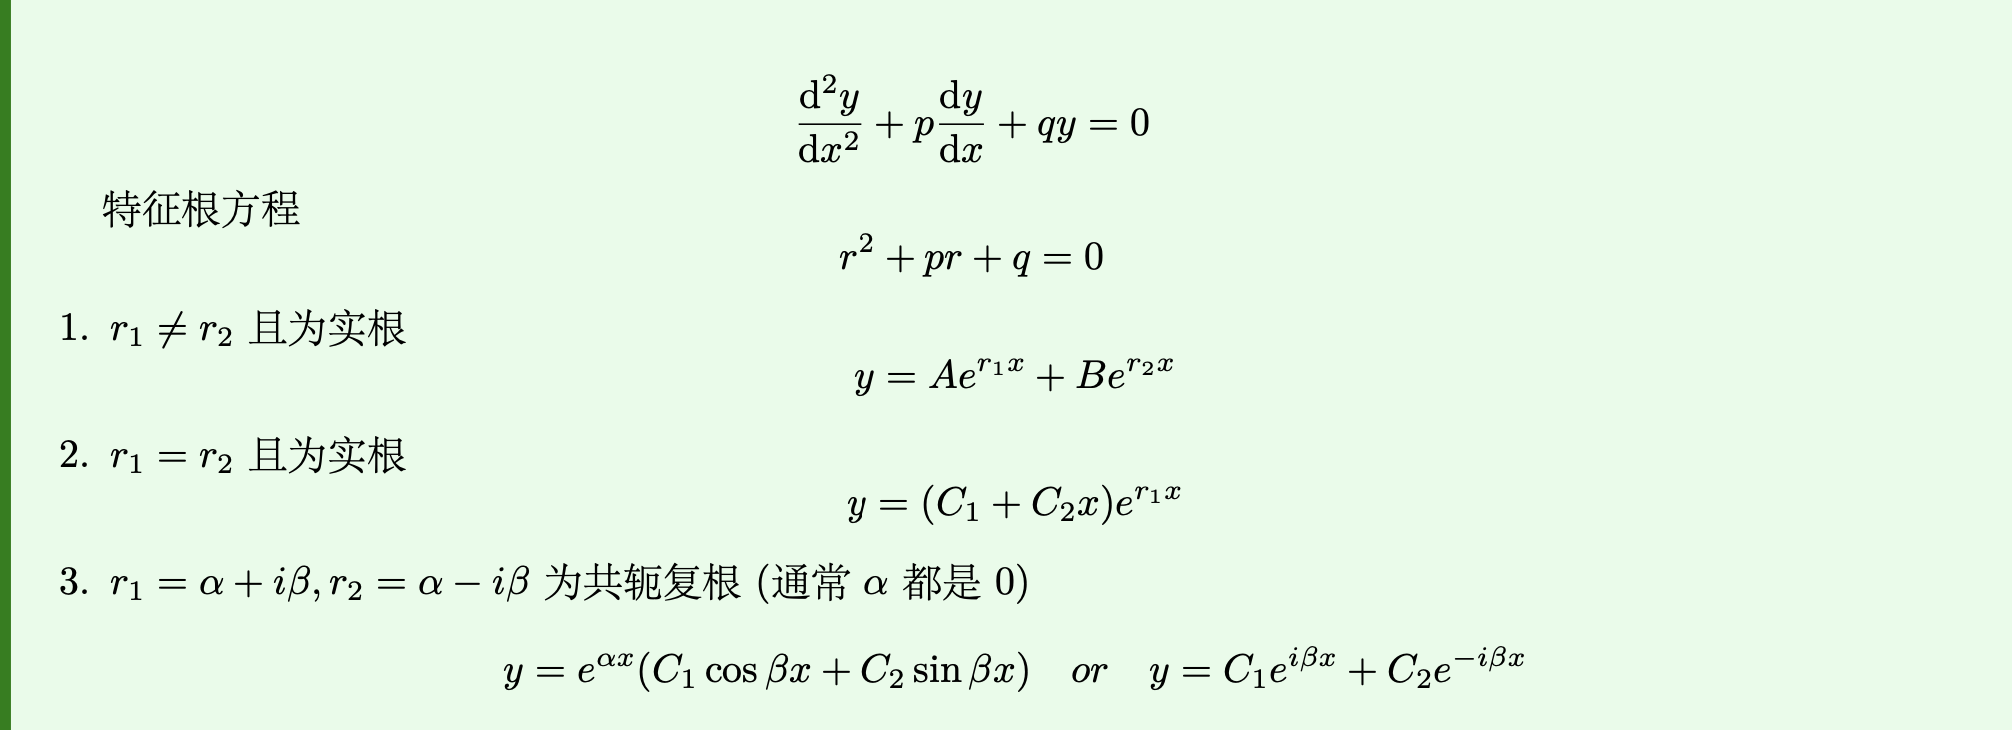
\includegraphics[width=\textwidth,keepaspectratio]{./pictures/1.3-10.png}
        \end{figure}

        
        \subsubsection{}
        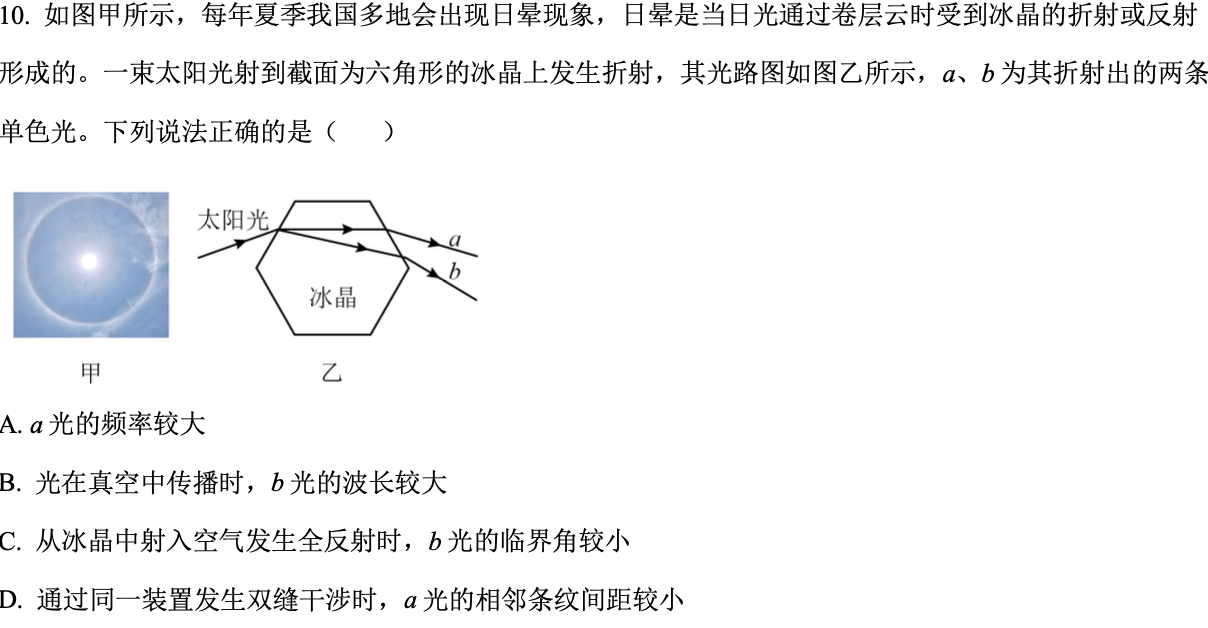
\includegraphics[width=50em,keepaspectratio]{./pictures/1.3-11.png}

        \begin{itemize}
            \item 正解:\quad C
            \item 总结:\quad 
            \begin{itemize}
                \item 光的\textbf{频率}$\nu$是本质属性,在任何介质下传播都不发生改变
                \item 同一介质中不同频率的光,\textbf{其折射率随频率单调递增}
                \item 同一光在不同介质的折射率不同
            \end{itemize}
            \item 扩展:\quad   
            \begin{formal}
                符号说明 
                
                \begin{tabular}{|c|c|c|c|c|c|c|c|c|c|}
                    \hline
                    频率 & 折射率 & 速度 & 临界角 & 波长 & 动量 & 干涉 & 能量 & 逸出功 & 逃逸光子动能   \\
                    \hline
                    $f$ & $n$ & $v$ & $C$ & $\lambda$ & $p$ & $\triangle x$ & $\varepsilon$ & $w_{0}$ & $E_{k}$   \\
                    \hline
                \end{tabular}

                \vspace*{2em}

                \begin{itemize}
                    \item 同一介质中不同频率的光  
                    
                    \vspace*{1em}
                    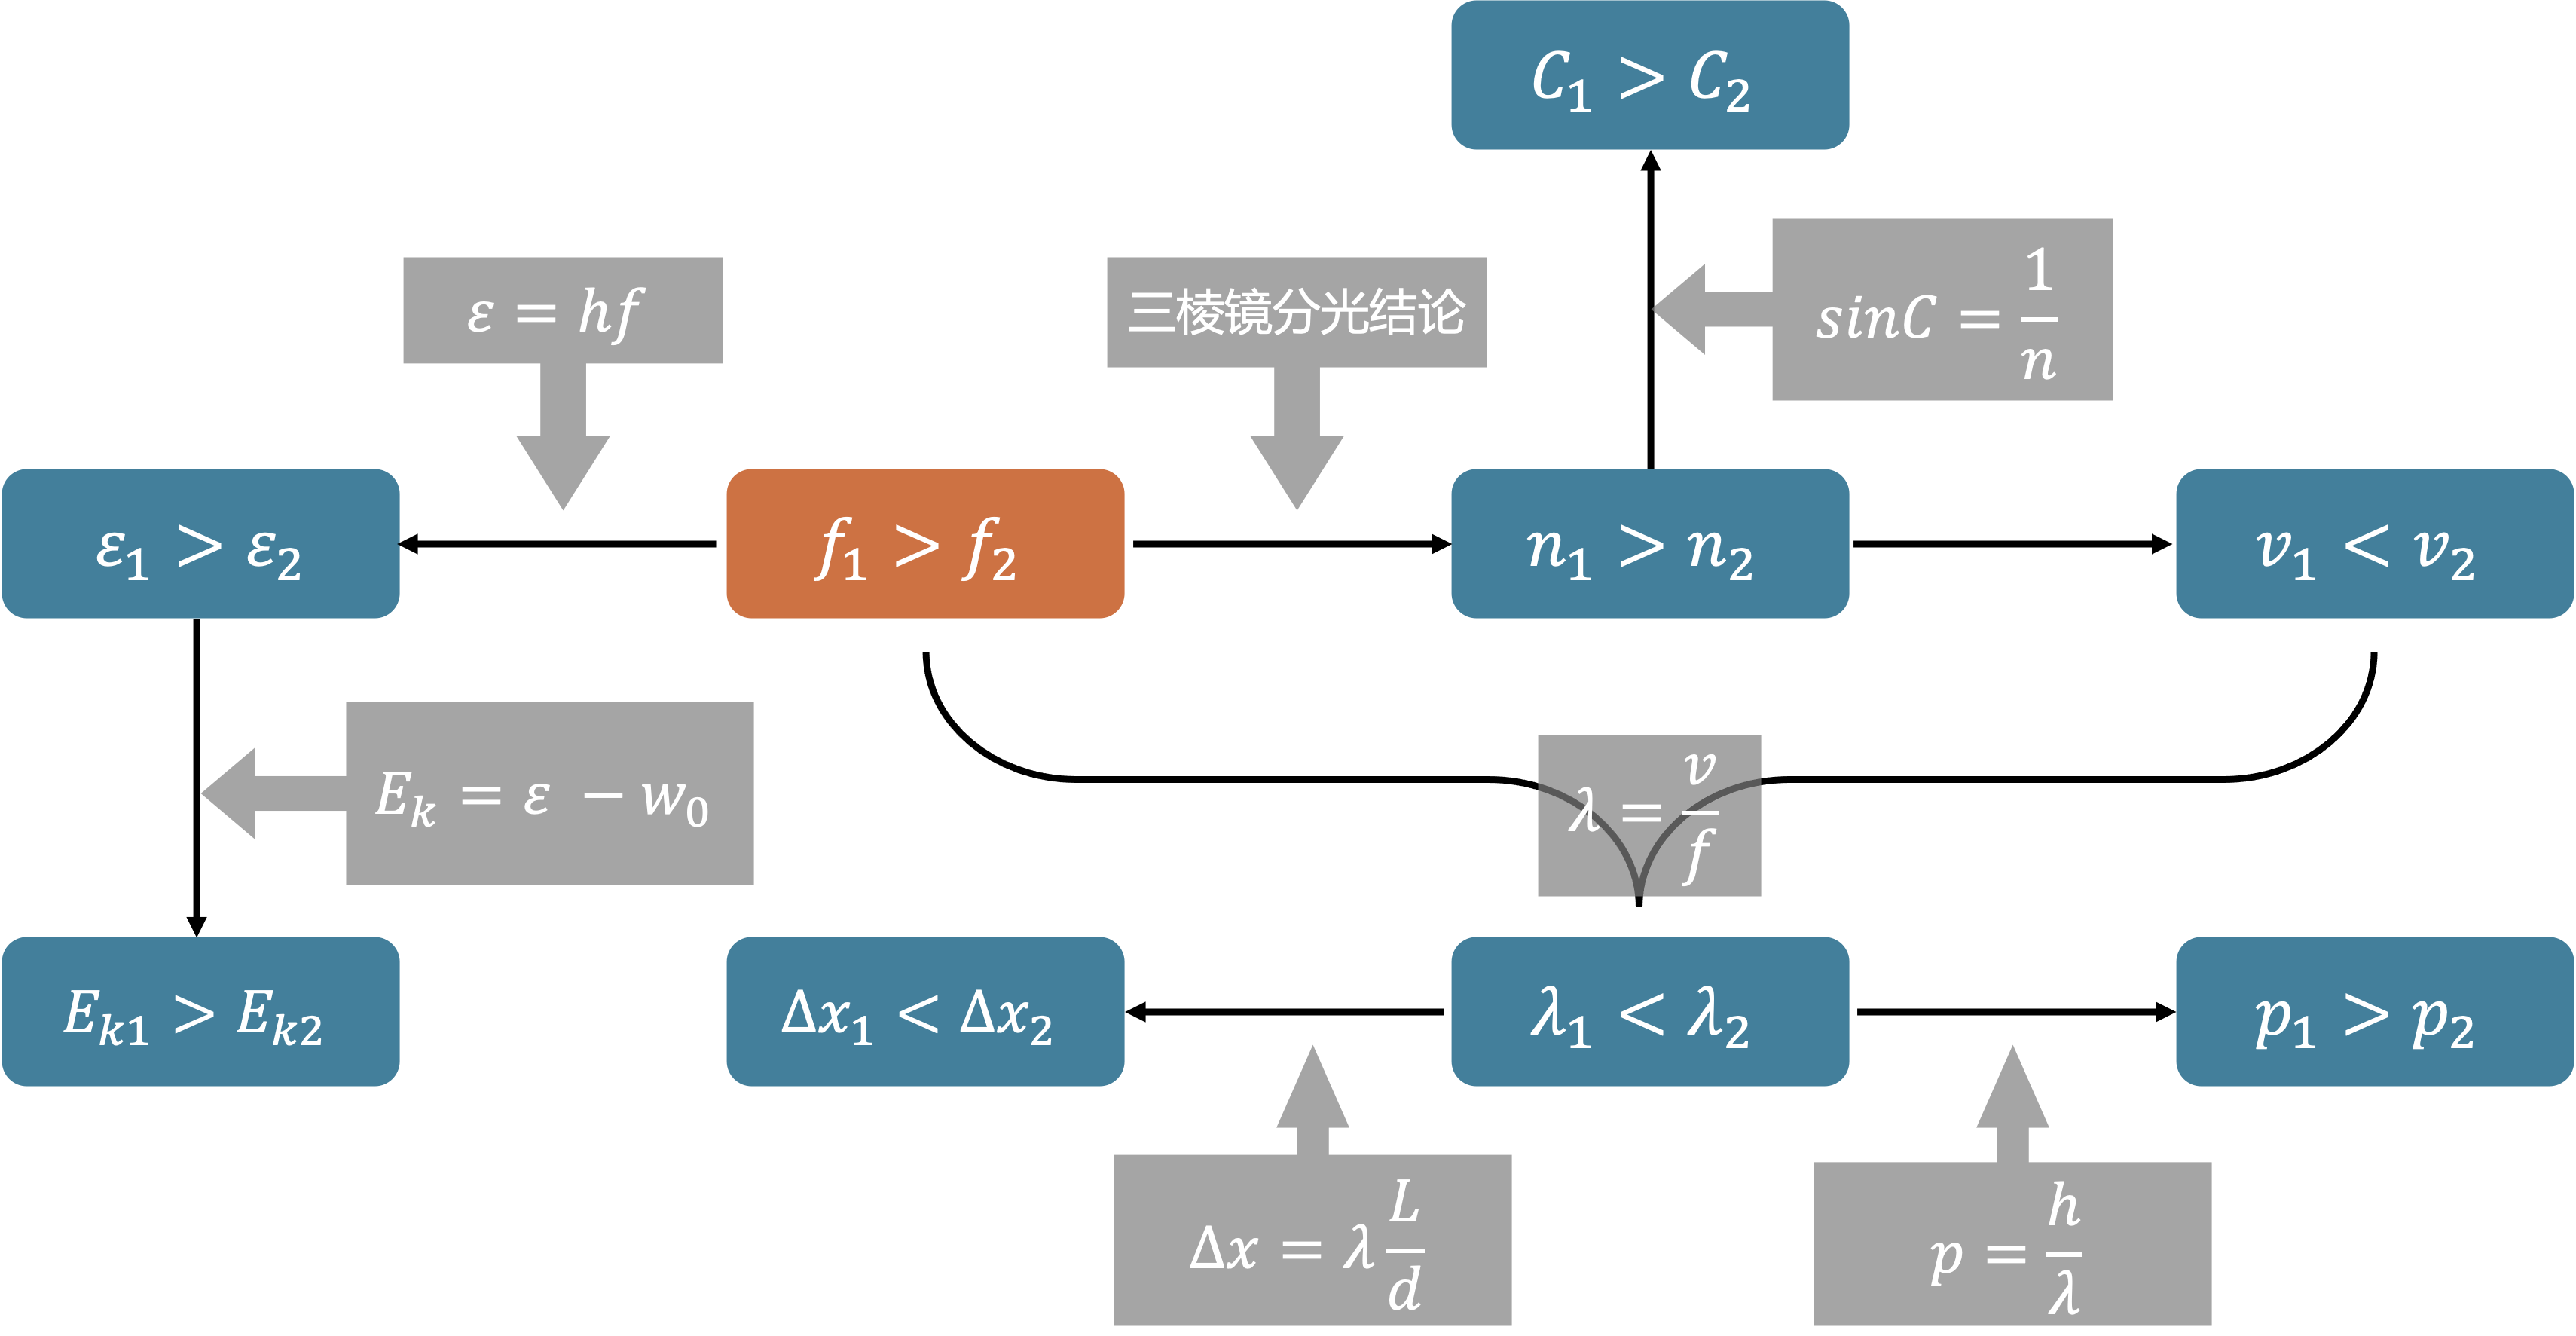
\includegraphics[width=40em,keepaspectratio]{./pictures/1.3-12.png}

                    \vspace*{2em}

                    \item 同一频率的光在不同介质(下标表示不同介质中)中
                    
                    \vspace*{1em}
                    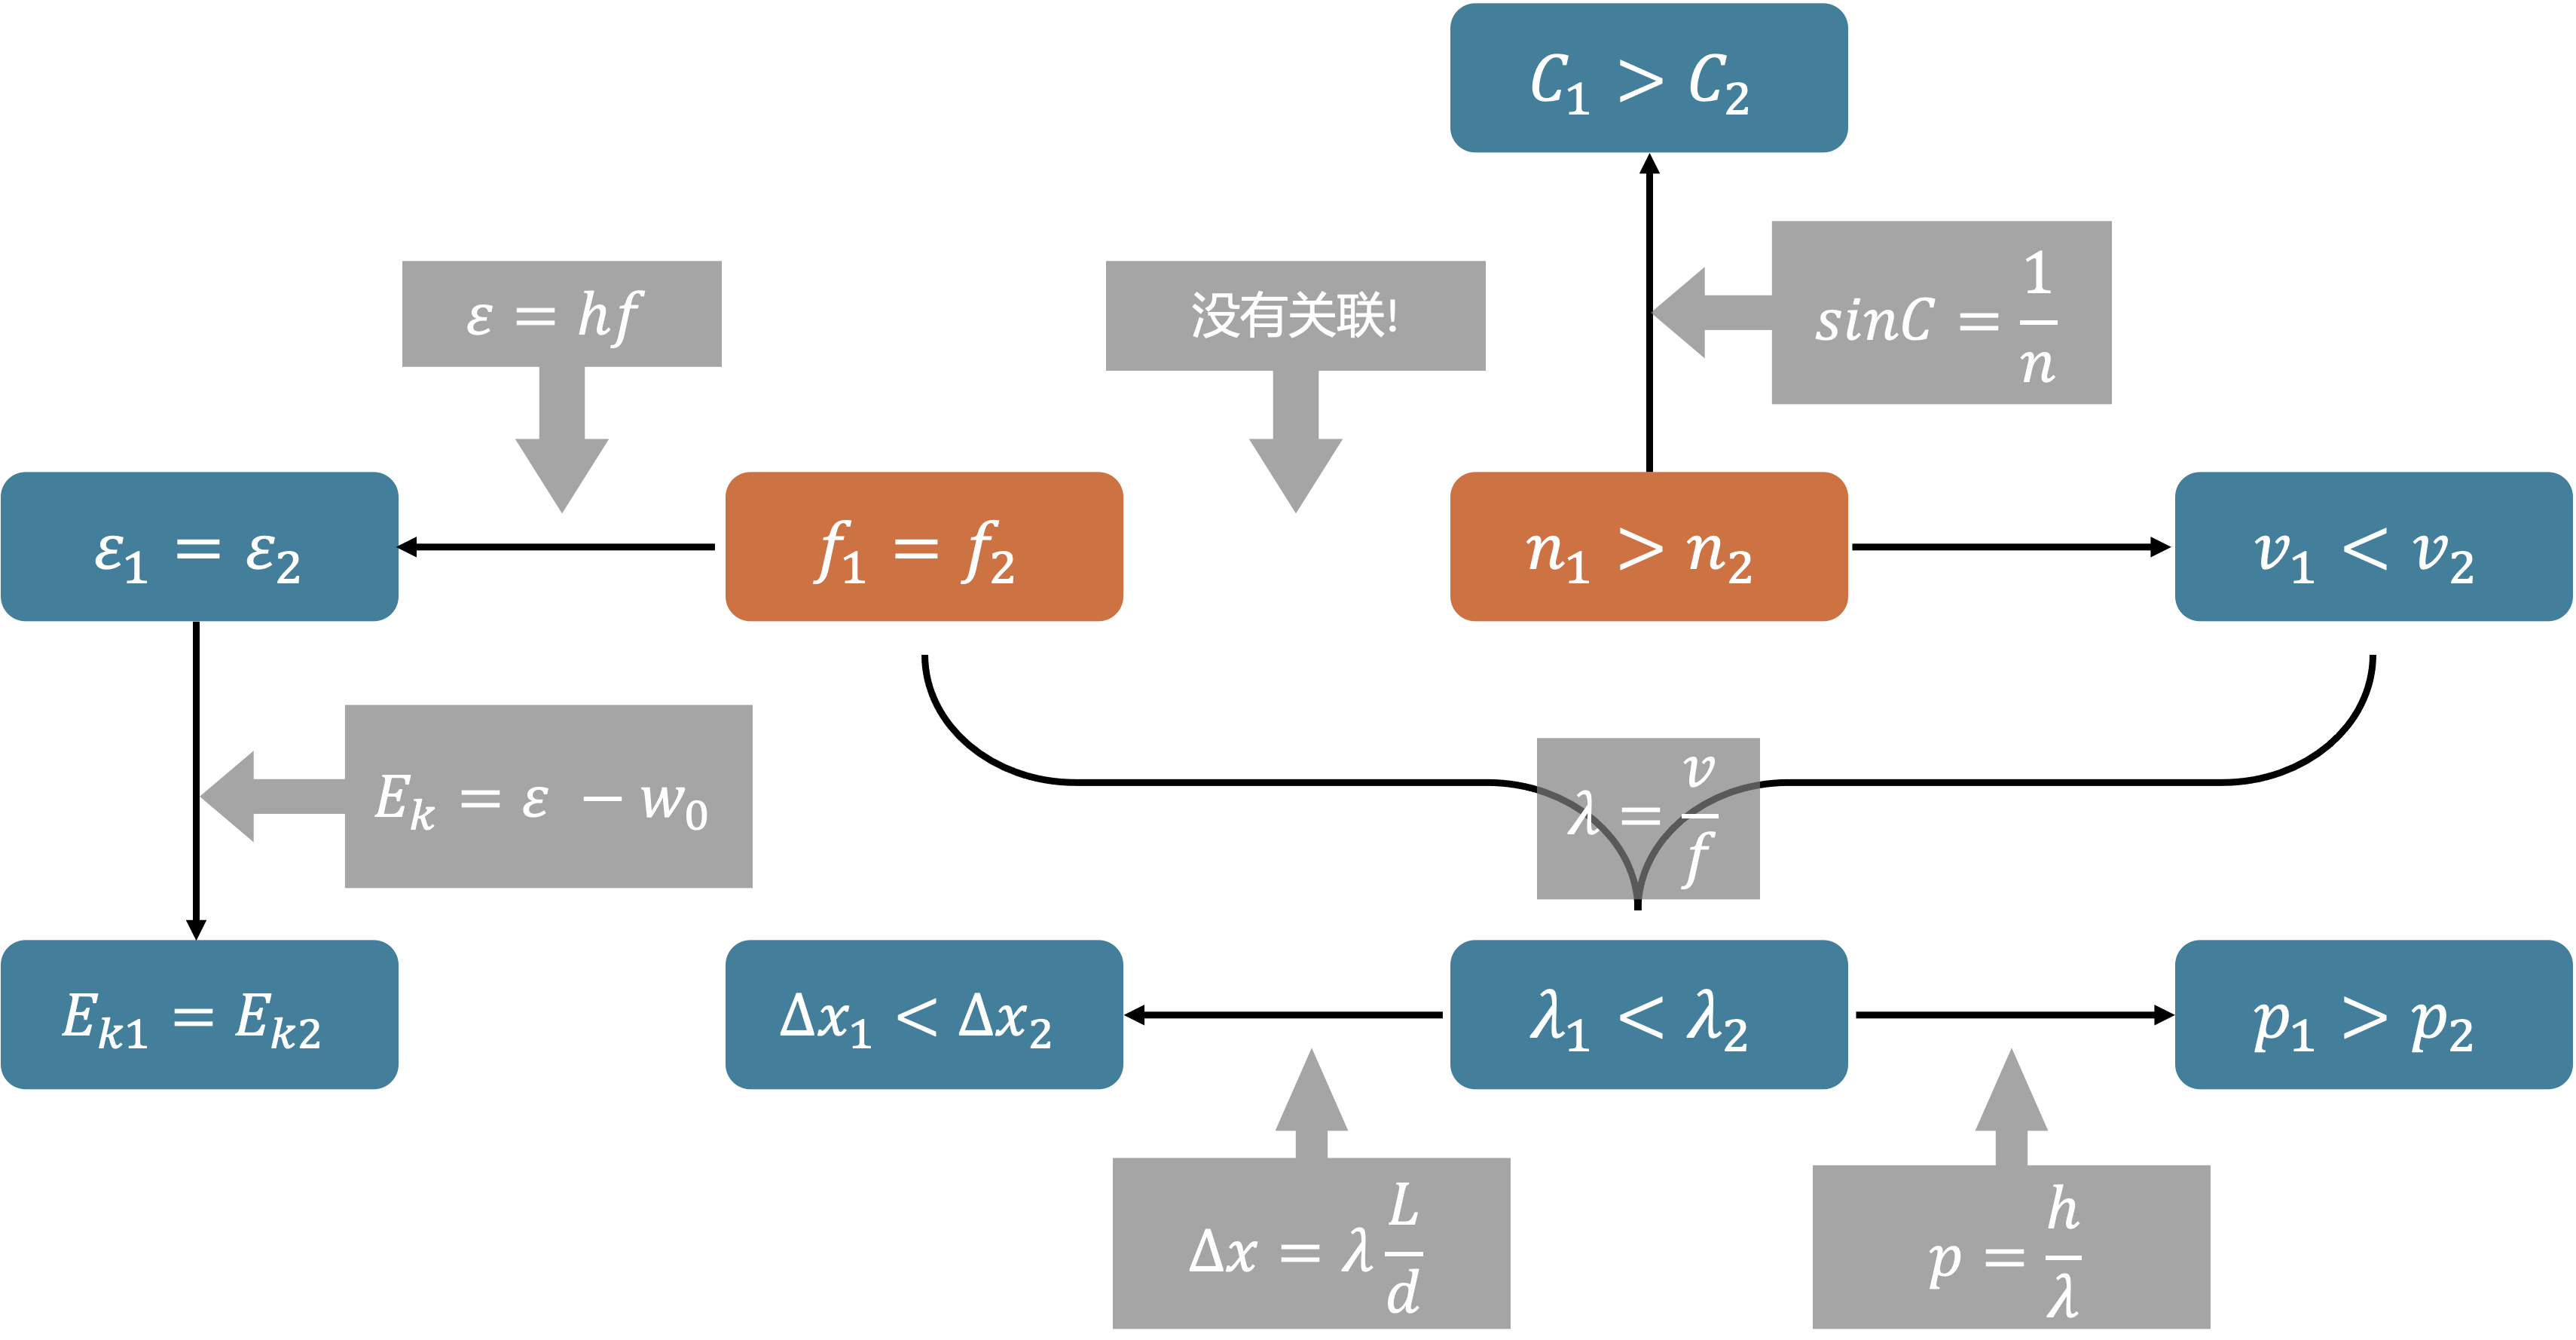
\includegraphics[width=40em,keepaspectratio]{./pictures/1.3-13.png}

                    
                \end{itemize}
            \end{formal}
        \end{itemize}
        

        

        
    


    \section{高二}





    \section{高三}







\end{document}